\ifdefined\included
\else
\setcounter{chapter}{5} 
\dominitoc
\faketableofcontents
\fi

\chapter{User Study to evaluate an integrated plan and execution scheme in simulation}
\chaptermark{User Study evaluating our approach}
\label{chap:6}
\minitoc

\section{Introduction}

To validate the approach presented in the previous chapter we conducted a user study on more than twenty participants. The purpose of this study is two-sided. 
First, we want to validate our overall planning approaches based on the proposed Model of Execution, and thus, show how it allows successful collaboration with a human. 
Secondly, we want to validate the Model of Execution itself, that is, showing how it allows the human to always be the leader and able to decide while the robot follows concurrently. We use a simple baseline to compare the Model of Execution with, and we show how our model allows to better satisfy human preferences and thus is preferred. 

We decided to conduct this study in simulation for various reasons. First, one of our assumptions is that all actions should roughly have the same duration. However, real-life robots are slow and not very reactive. Those aspects may bias the results of our study which is focused on decision-making. Secondly, simulation allows several simplifications that are acceptable for study. Collision with the cubes has been disabled to make the robot faster both in planning and executing its arm movements. In addition, simulation allows having a perfect perception of the environment. In a real-life experiment, perception errors may occur leading to replan, and thus slower execution, or even wrong decisions. Moreover, our model assumes that both agents synchronize after each step. Hence, it was easy in simulation to prevent the human from acting too soon and synchronize automatically their actions. In a real-life scenario, we couldn't physically prevent the participant from acting. This would imply a heavier training process for the participants to avoid desynchronizing with the robot. In practice, an additional execution supervisor should be developed to permit desynchronizing as long as they are not too big, and hence, prevent the system from crashing. This would require a significant technical effort to implement.

To conduct this study I developed a dedicated interactive simulator using a Tiago robot. In addition, the automaton described by the MoE has been implemented and integrated with the simulator to provide a proper execution and supervision scheme. Eventually, through carefully designed scenarios and using a shortened version of the PeRDITA questionnaire~\cite{devin_evaluating_2018} we gathered the feelings and impressions of the participants regarding the different robot behaviors. We also recorded logs from each executed scenario allowing us to draw a timeline of the execution and compute objective metrics for each scenario among which can be found: the time to complete the task, the human decision time, or the time for the human to be free. Several relevant facts and conclusions can be extracted from the collected results and are discussed in this chapter.

This chapter is organized as follows. First, the interactive simulator functionalities and operations are described. Then the methodology of the user study is provided along with anonymous information on the participants. After, the results obtained are presented and then discussed, validating the proposed hypothesis.

****

why simulation: HRI rebuttal: we rely on a reactive execution, real life robot are slow and not very reactive, may have perception errors, thus may bias our results focused on decision making.

Thus, we developed an interactive simulator running robot policies generated as explained the Chapter~\ref{chap:4}. Then, we conducted a user study using this simulator.

The purpose of this study is two-sided. First, we want to validate our overall planning approaches based on the proposed Model of Execution, and thus, show how it allows successful collaboration with a human. Secondly, we want to validate the Model of Execution itself, that is, showing how it allows the human to always be the leader and able to decide while the robot follows concurrently. Compared to a simple baseline, we also want to show how this model allows to better satisfy human preferences and thus is preferred. 

This chapter is organized as follows. First, interactive simulator functionalities and operations are described. After, the study protocol is presented as well as some analysis of the participants. Eventually, the obtained results are presented and discussed.

% *****

% Objective of the study is to validate the following:

% \begin{itemize}
%     \item \textbf{Overall planning and the use of Model of Execution during planning}: Always reach the goal, with different preferences, no need of prior negotiation, overall positive interaction, simple, use of MoE allows to explore all possible execution traces and complete the robot policy allowing human free to choose any action (OptimalRatio < 1.0) while still having a reactive robot, step synchronization questionable (sometimes liked, helps participant. Sometimes a bit lost in the step, however still ok.), real scenario should use additional execution supervisor allowing step superposition.
    
%     \item \textbf{Use of Model of Execution during execution}: The MoE describes how the robot always acts in a concurrent and compliant manner with the human. This allows the human to always (at every step) be in control. By using a mirror baseline where the robot always takes the lead instead of being the follower, we show that having the robot as a follower is preferred (H feels in control) and allows for better satisfying human preferences. The drawback of this approach is that currently, the robot is always a follower, making it slower since it always waits for the human to do something to adapt and act. Given to good results of the RF (with correct estimation) the question arises of trying to mix both approaches, having a robot that is by default a follower but sometimes takes the lead to be faster (when no risk of conflict?)
    
%     \item \textbf{Neither HA-planning nor compliant execution are sufficient alone}: Indeed, when the robot follows the HF regime with an incorrect estimation of human preferences the human can ``impose'' their decisions on the robot which will adapt, and thus, the human can satisfy their preferences anyway. However, in such scenarios, the human usually have one chance to impose their decision. Hence, if they are distracted the robot will eventually act in a not desired way which can lead to negative interaction. This can be observed with some participants either getting confused or distracted, and this didn't happen when the robot had a correct estimation of human preferences. Hence, it is important to have both a pertinent robot policy/plan selection complemented with an adaptive and compliant execution to have the best interaction possible.
    
%     \item \textbf{Not investigated in this work but,} our approach has been designed to allow specifying online new human preferences, updating the whole robot policy to satisfy the new given preferences. This allows either the human to directly specify their intents and preferences to the robot, or, an external process estimating online the human preferences.
% \end{itemize}

% The goal is to validate our approach presented in the previous chapter and justify the following. We believe that the robot should plan its actions with a compromise of optimizing the task efficiency, maximizing social criteria and satisfying human preferences while collaborating with humans. However, satisfying those social criteria is challenging since they cannot be accurately quantified. Especially for human preferences which can fluctuate a lot depending on their mood and context. That is why we believe, in addition to planning the best course of action using all these criteria, it is relevant or even mandatory for the robot to adapt and be compliant with human online decisions and actions. 

% Hence, this study aims to show two main things. First, during execution, the robot should adapt and be compliant with the human actions. Indeed, it is hard to accurately estimate human behavior and preferences. In case of incorrect estimation, having a compliant robot helps to satisfy the human preferences (HF vs RF, better answers). Also, the human may act differently than expected by the robot, the latter should be able to allow this and comply with it (ratio\_h\_optimal < 1.0).
% Secondly, the study validates our overall planning (and execution?) approach. The goal is always solved. The collaboration is always useful (more or less) and not so low (positive). 
% Third, we can also say that despite having to be compliant online, it is very beneficial to plan correctly beforehand the robot actions. 

% \textbf{TODO: GOAL of the study is to validate two things. First, our overall planning approach. Secondly, the HF model of execution. 1) Should see that overall even when wrong RF the robot isn't so bad, still useful, simple, competent, responsive. Could do better and a bit frustrating but still ok to accomplish the task. 2) Should see that HF is significantly preferred and results in more acceptable and appreciated behavior : Adaptive, Appropriate, Accommodating, Positive.}

\section{Related work}

\subsection{Questionnaires}
Many questionnaires are used in the field of HRI. The main ones are listed here: GodSpeed, HRIES, PeRDITA, RoSAS, and Trust Perception Scale-HRI. 

Each questionnaire has specificities and helps to measure certain aspects of the robot. Many include appearance items to evaluate the look of the robot. Since our focus is on robot decision-making, we decided to base our questionnaire PeRDITA. Indeed, this questionnaire has been designed to evaluate the pertinence of robot decisions in a Human-Robot Joint Action Context, which is exactly our case. Yet, the full questionnaire is a bit heavy and also covers communication which isn't our topic in this work. 
That is why we decided to shorten the questionnaire by removing the section on communication and a few redundant items. Redundant items are helpful to evaluate the consistency of a questionnaire and this has already been done in~\cite{devin_evaluating_2018}. Hence, to avoid participants getting bored and lost by filling out the whole questionnaire after every scenario we kept 12 items covering the following dimensions: robot perception, interaction, collaboration, and acting.



\section{Study protocol} \label{sec:study_protocol}

Methodology: 
Initial demographics questionnaire to identify potential individual difference ratings. Then, presentation instructions/text. After, familiarized with the simulator through an interactive tutorial. Eventually, the six scenarios in randomized order are experienced by the participant. After each scenario, the participant answers a shortened version of the PeRDITA questionnaire and logs about the execution are saved. Eventually, the participant is asked about their overall impressions regarding the interaction they had with the simulated robot, and they are asked which scenario they preferred the most and the least. The overall experiment takes about 35-40 min per participant. 

objective, participants, material, experiment design, procedure, measures

This section describes the objectives and protocol of this study.  



\begin{figure}
    \centering
    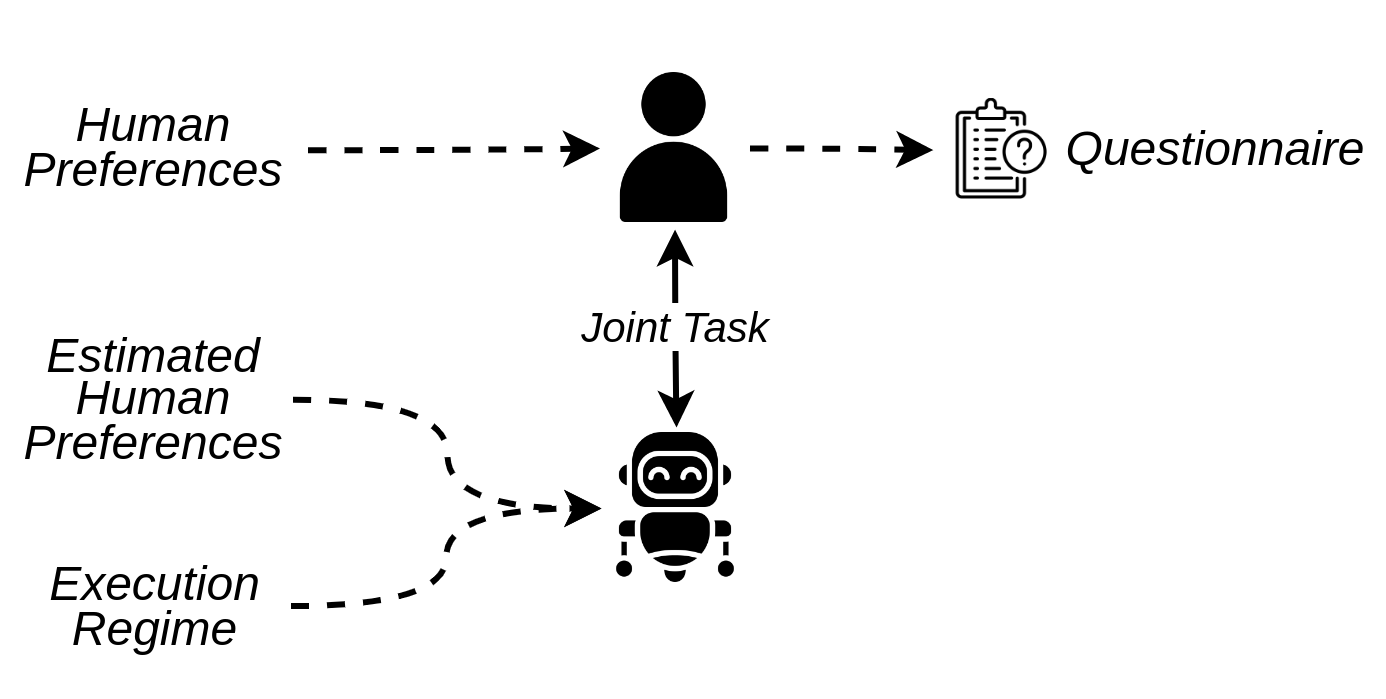
\includegraphics[width=0.8\textwidth]{Chapter6/UserStudyProcedure.png}
    \caption{A scenario of the User Study Protocol. Each participant goes through 6 scenarios and answers 6 questionnaires to evaluate each different robot's behavior}
    \label{fig:user_study_protocol}
\end{figure}




Through this study we want to demonstrate the benefits of using the model of execution described in the previous chapter~\ref{chap:4} in a collaborative context. We believe this model of execution is pertinent to be taken into account when executing and supervising a robot's plan. For the same reasons we based the policy generation of this model and aim to justify our choice and validate our approach.

In this study, each participant is made to collaborate six times with a simulated robot to achieve a shared task, each time is referred to as a scenario. The robot exhibits a different behavior in each scenario. After each scenario, the participant evaluate the robot's behavior through the PeRDITA questionnaire \cite{devin_evaluating_2018}.

Beforehand, every participant answers a few general/demographic questions and is familiarized with the simulator functionalities through an integrated tutorial. Only then they start the six consecutive collaborative scenarios, answering every time a questionnaire to describe the interaction. Eventually, every participant is asked to share their general feelings and impressions about the overall interaction with the simulated robot, and they are asked to tell which scenario they preferred the most and the least.

\begin{figure}
    \centering
    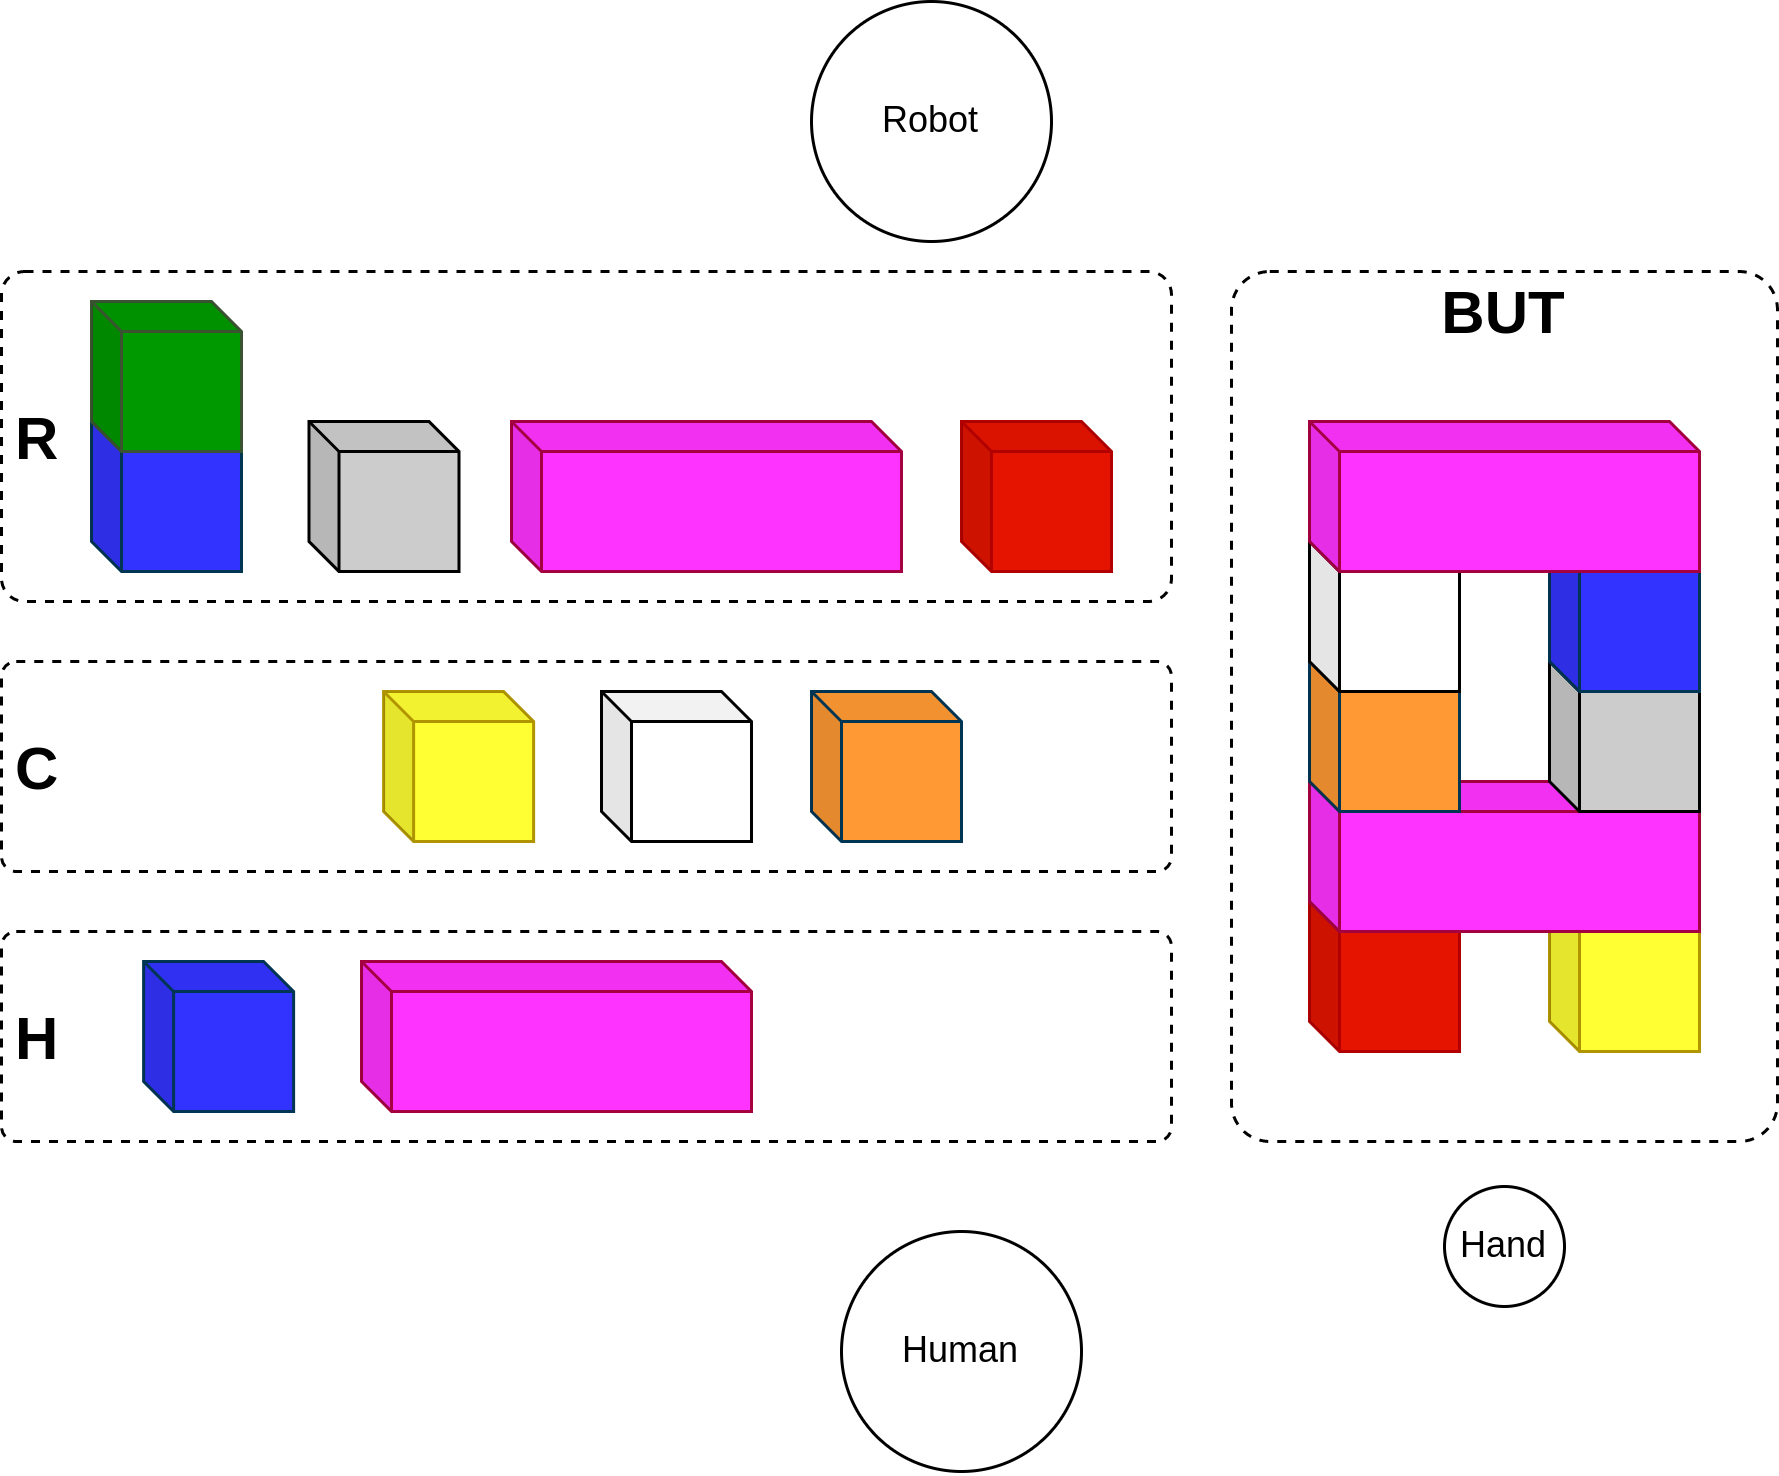
\includegraphics[width=0.8\linewidth]{Chapter6/task_description_study.png}
    \caption{Description of the shared task to achieve in the study.}
    \label{fig:task_description_study}
\end{figure}

We now provide details about the task, the scenarios and how the different robot behavior are generated. 
The shared goal, which is stacking the cubes to match the given pattern, remains the same in all scenarios. The cube disposition on the table also doesn't change either. The task description is depicted in fig~\ref{fig:task_description_study}. For this problem, our planning approach generated a solution graph with 700 PStates/nodes leading to 6 different final states/leaves. This solution graph comprises $6839430$ different possible courses of action. The length of the plans is about $19.77 \pm 1.59$ steps, with a minimal length of $11$ steps and a maximal length of $23$ steps.

To progress in the task, the agents can perform three different primitive actions which are the following: \textit{pick} a cube, \textit{place} a cube in the stack, or, \textit{drop} a cube back on the table.
These actions have a few preconditions, more or less intuitive, that are communicated and experienced by the participant during the integrated tutorial.
First, one can \textit{place} a cube if they hold the cube, and if the targeted location is free and supported. That is, the cubes directly below the targeted location must be placed before being able to place a cube in the targeted location.
Secondly, one can only \textit{pick} a cube from their respective reachable zones of the table, i.e., Human and Center zones for the human, and Robot and Center zones for the robot. Also, one can only pick a cube if it can be placed immediately. Thus, one cannot pick a cube ``in advance'' and has to wait to its placement condition to be true before picking it up. For instance, both pick bars can only be picked up after the yellow and red cubes have been placed. This rule helps to create interaction conflicts serving the purpose of this study. Moreover, although the participants find this not intuitive they get used to it really fast and this feeling seems to be significantly reduced along the experiment.
Third, one can \textit{drop} a cube back on the table only if they hold it and if it cannot be placed.

For each scenario the participant is given instructions regarding how to solve the task. The participants are asked to consider these instructions as their own choice and preferences regarding the task resolution, and thus, to act accordingly while collaborating. The instructions at each scenario are one of the two following.
On the first hand, the participant shall act in a way to finish the task as soon as possible. Here, it consists in trying to perform as many actions in parallel as possible to progress faster. These preferences are latter referred to as Task End Early (TEE).
On the other hand, the participant shall act in a way to be freed as soon as possible. That is, they should finish their mandatory part of the task as soon as possible, so they could leave and let the robot finish alone. Here it consists in placing the pink bar from the Human zone as soon as possible. These preferences are latter referred to as Human Free Early (HFE).
On its side, the robot doesn't directly have access to these instructions/preferences, they are only estimated. Hence, for each scenario, the robot is given a more or less accurate estimation of the human preferences that are communicated to the participant. Note that the participants aren't aware that the robot has an estimation of their preferences, neither that this estimation can be inaccurate.
This way, we created three scenarios with different pairs of human preferences and associated estimation. In the first pair, the human shall finish the task early and the robot has a correct estimation, i.e., the robot's policy is helping the human to finish the collaborative task early. In the second pair, the human preferences remain the same, but the robot estimation is incorrect. The robot is trying, mistakenly, to minimize the human effort. As a consequence, the robot tends to pick cubes that the human could pick, preventing the human from acting and making the task completion longer. In the third pair, the human shall free themselves early, but the robot estimation is again erroneous. The robot will try to finish the task early while its priority is to place the first pink bar, which is conflicting with the given human preferences.

Additionally, in each scenario, the robot follow one of the two following execution regimes:
\begin{itemize}
    \item \textbf{Robot-First (RF)}: the robot always initiates actions first, and the participant take action afterwards.
    \item \textbf{Human-First (HF)}: the robot always lets the participant take the initiative, and then acts.
\end{itemize}
The \textit{Human-First} execution regime corresponds to the Model of Execution described in the previous chapter. At each step, the robot waits for the human's decision and will execute the best action that complies with it. The human always start acting first and the robot follows. On the other hand, the \textit{Robot-First} regime corresponds to a naive and straightforward policy execution where, at each step, the robot directly starts executing the overall best robot action given by the policy. The robot always starts acting forcing the human to comply. The \textit{Robot-First} regime serves as a baseline to evaluate the proposed \textit{Human-First} regime, described by our Model of Execution and used in the policy generation.
Eventually, we associate each of the three previous pairs of preferences and estimation with one of the two different execution regime. As a result, we obtain six different scenarios with six different robot behaviors named in table~\ref{tab:scenario_names}.

\begin{table}
    \caption{Name of the six scenarios. 
    Columns represent the preferences/estimation pairs and the rows correspond to the execution regimes.}
    % \vspace{-15pt}
    \begin{center}
    \begin{tabular}{c|c|c|c|}
        \cline{2-4}
                                                & Pair A        & Pair B            & Pair C\\
                                                & TEE: correct  & TEE: incorrect    & HFE: incorrect\\
        \hline
        \multicolumn{1}{|c|}{Human-First}       & S1            & S3                & S5\\
        \hline
        \multicolumn{1}{|c|}{Robot-First}       & S2            & S4                & S6\\
        \hline
    \end{tabular}
    \end{center}
    \label{tab:scenario_names}
\end{table}

Note that our goal is to evaluate and compare the different robot behaviors. However, at the beginning, the participants don't have any references to compare with which can influence their answers in the very first scenarios. One solution is to ask the participants to answer all six questionnaires at the end, after being familiar with the six scenarios. We consider that this option demands a too heavy mental workload to recall accurately each specific scenario, and may bias the answers. As a consequence, we decided to ask the participants to answer the questionnaire after each scenario as a draft. During the experiment, they can rectify their answers to match more accurately their feelings. At the end, using the drafts, they share their final answers for each scenario. We believe this process allows to more accurately gather the feelings of the participants. Moreover, the ordering in which the participants encounter the scenarios is uniformly randomized to prevent any order effect. 


\begin{table}[h]
    \footnotesize
    \begin{tabular}{ccc}
    \hline
    \textbf{Dimension}                         & \textbf{Question}                                                                                                                     & \textbf{Item}             \\ \hline
    \multirow{3}{*}{\textbf{Robot perception}} & \multirow{3}{*}{\begin{tabular}[c]{@{}c@{}}In your opinion,\\ the robot is rather:\end{tabular}}                                      & Apathetic/Responsive      \\
                                               &                                                                                                                                       & Incompetent/Competent     \\
                                               &                                                                                                                                       & Unintelligent/Intelligent \\ \hline
    \multirow{3}{*}{\textbf{Interaction}}      & \multirow{3}{*}{\begin{tabular}[c]{@{}c@{}}In your opinion, the interaction\\ with the robot was:\end{tabular}}                       & Negative/Positive         \\
                                               &                                                                                                                                       & Complicated/Simple        \\
                                               &                                                                                                                                       & Ambiguous/Clear           \\ \hline
    \multirow{3}{*}{\textbf{Collaboration}}    & \multirow{3}{*}{\begin{tabular}[c]{@{}c@{}}In your opinion, the collaboration\\ with the robot to perform the task was:\end{tabular}} & Restrictive/Adaptive      \\
                                               &                                                                                                                                       & Useless/Useful            \\
                                               &                                                                                                                                       & Inefficient/Efficient     \\ \hline
    \multirow{3}{*}{\textbf{Acting}}           & \multirow{3}{*}{\begin{tabular}[c]{@{}c@{}}In your opinion, the robot\\ choices of action were:\end{tabular}}                         & Inappropriate/Appropriate \\
                                               &                                                                                                                                       & Annoying/Accommodating    \\
                                               &                                                                                                                                       & Unpredictable/Predictable \\ \hline
    \end{tabular}
    \caption{PeRDITA Questionnaire: Participants have to place themselves between the two antonym items in a scale of 7.}
    \label{tab:perdita_questionnaire}
\end{table}

The questionnaire filled by the participants after each scenario is a shorten version of the PeRDITA questionnaire, and its items are gathered in table~\ref{tab:perdita_questionnaire}. 
In addition to the questionnaires, for each scenario, the interactive simulator produces logs from which we extract several metrics and an overall timeline of the execution. The timeline depicts the activities and actions of each agent along the task progression. The subjective measures done through the questionnaire are complemented with the objective metrics extracted such as the duration to complete the task, the number of human actions, the total duration of human inactivity, and more. 


There are a few restrictions on the actions that can be performed. First, an agent can only pick cubes that can be placed immediately. This means that agents cannot pick cube in advance to anticipate each other's actions. Allowing such behavior could generate a very interesting scenario. However, here we want to purposely generate some conflicts to evaluate the robot's behavior and reactions. Without this restriction, the agents would have too much flexibility in their actions and decisions which makes it harder for the conflicts to happen.  
Additionally, when holding a cube, the agents can only place the cube in the stack on back to its original place. As a result, the agents cannot displace the cube on the table to make them reachable to the other agent. This restriction has been added for the same reasons as the first one and simplifies the conflicts generation. 

\begin{figure}
    \center
    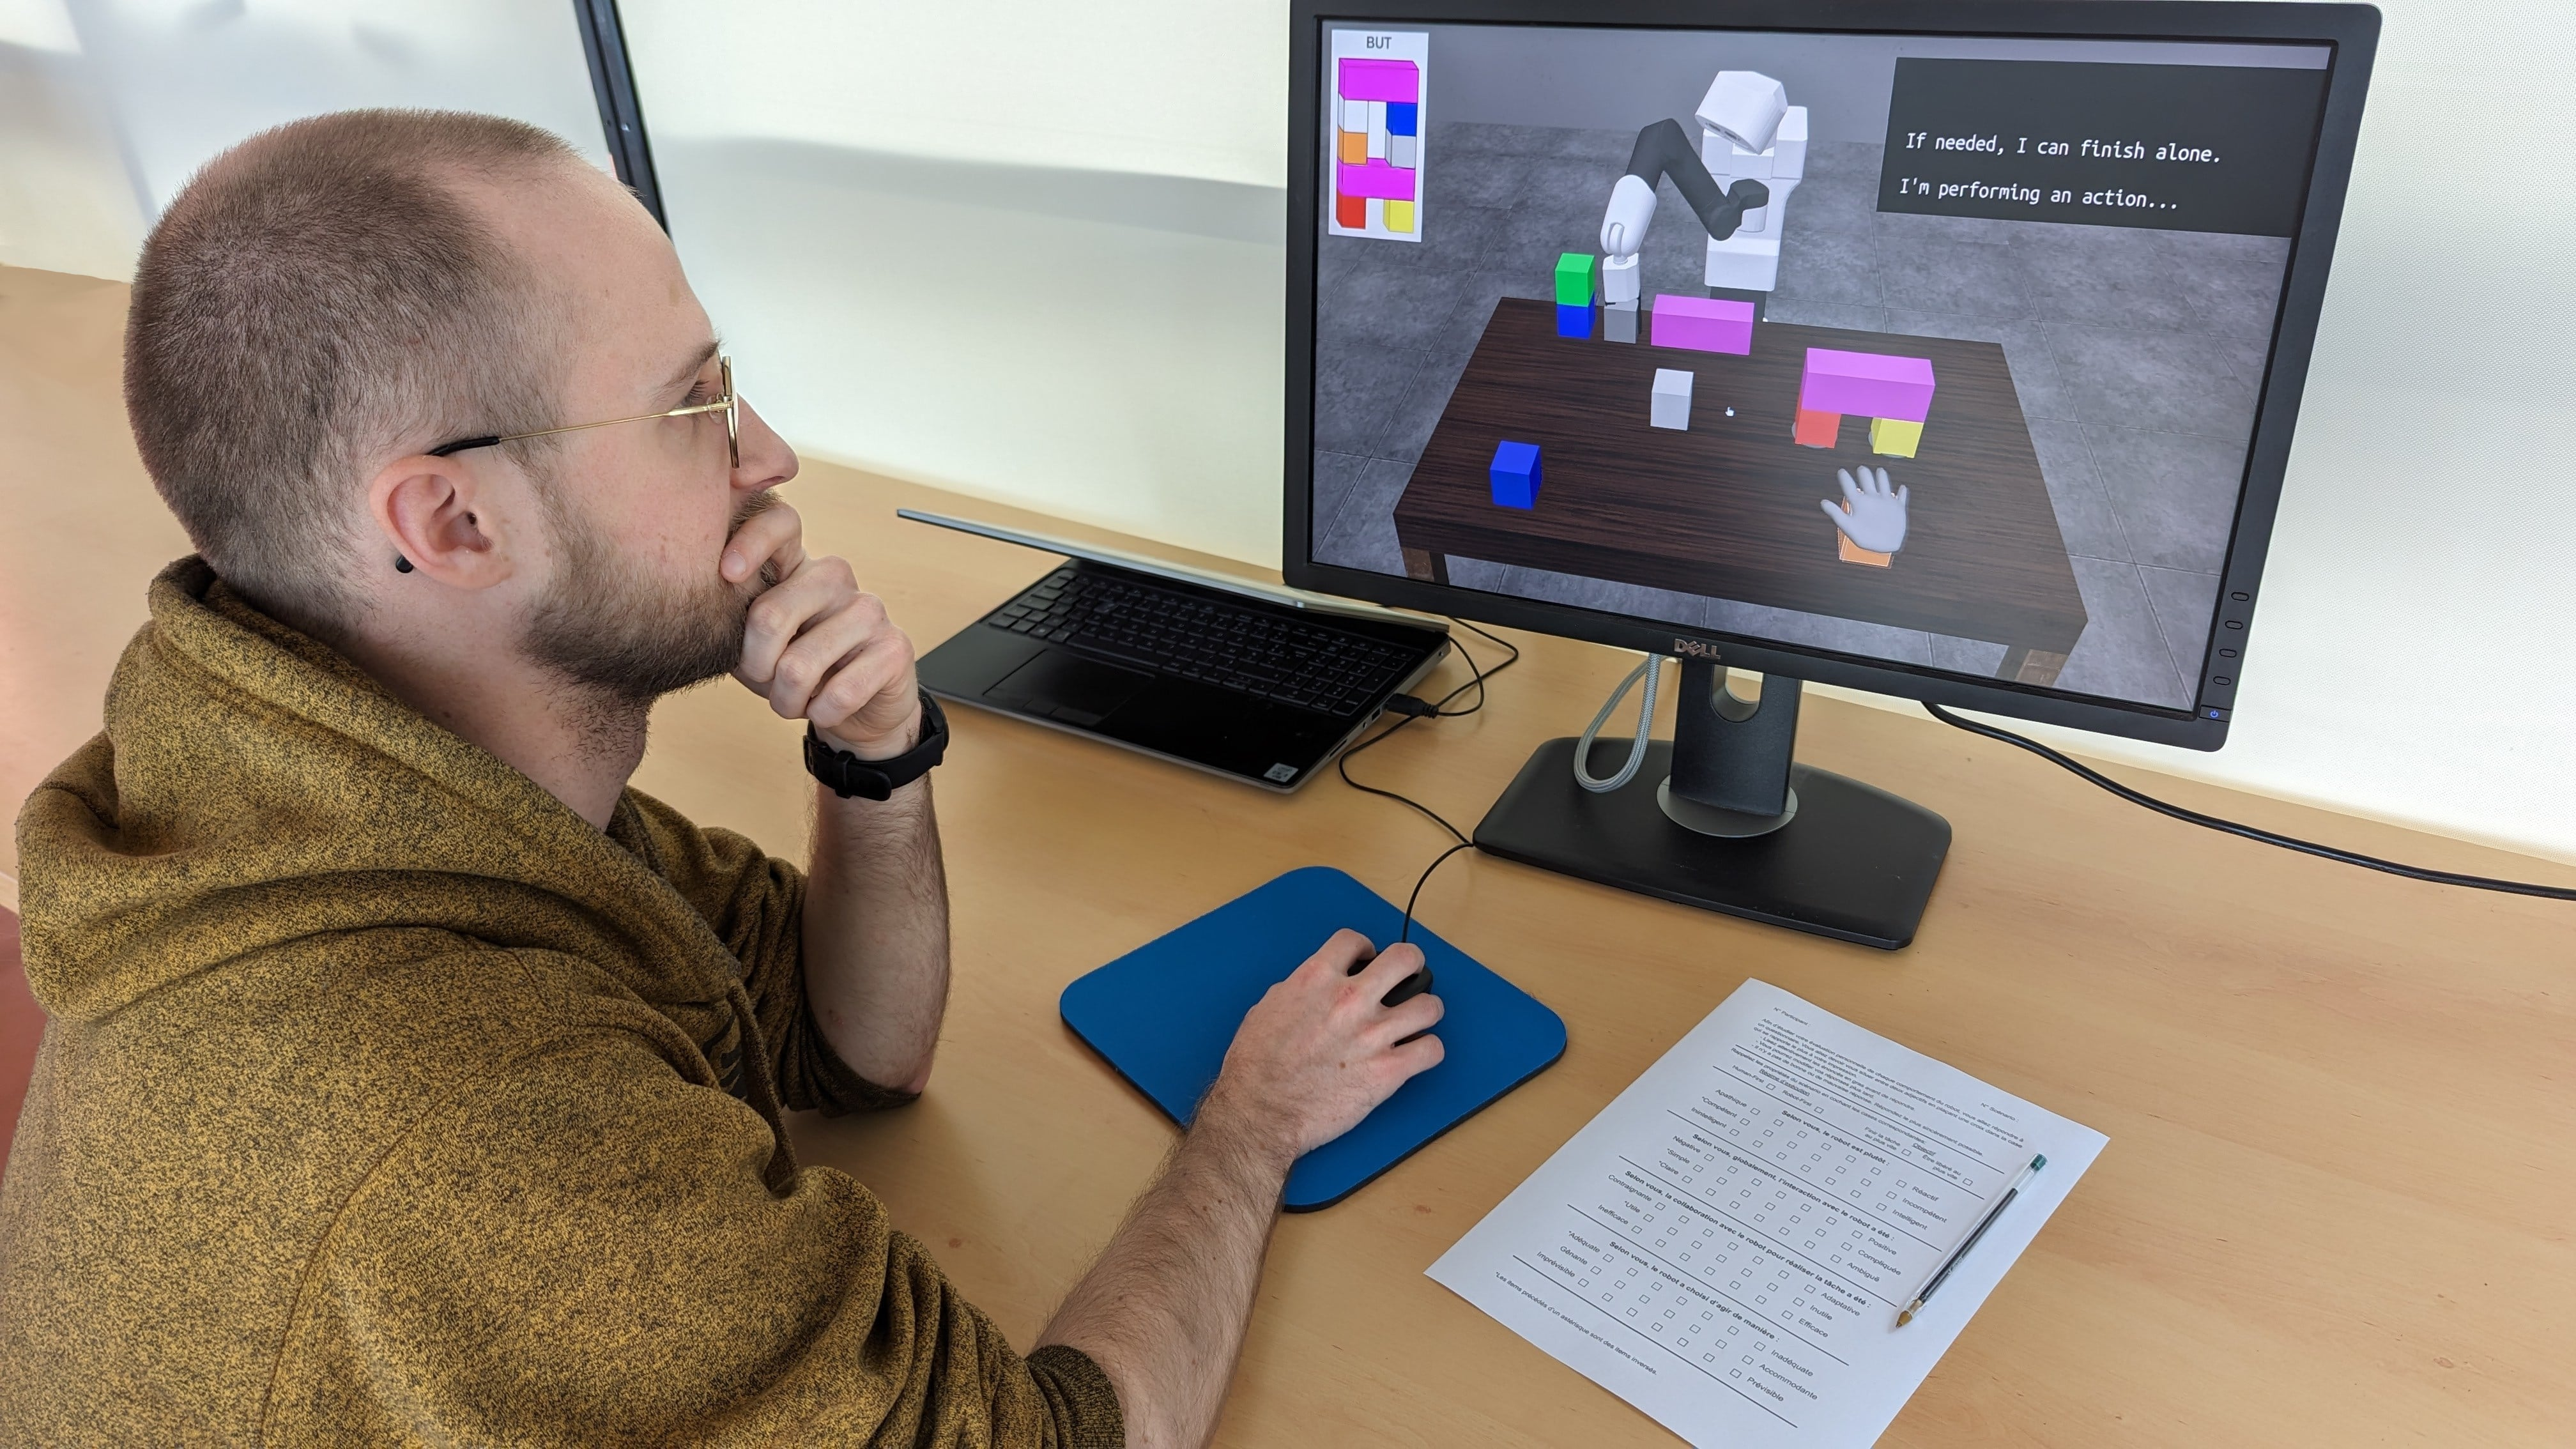
\includegraphics[width=\linewidth]{Chapter6/participant-min.jpg}
    \caption{One scenario execution where a participant is collaborating with the simulated robot using the mouse. Once the task is completed, the participant is asked to fill the questionnaire on the desk with a pencil to transcribe their impressions.}
    \label{fig:participant}
\end{figure}

The participants were collaborating with the robot using a mouse. The simulation was run on a laptop connected to a bigger screen allowing participants to see clearly the simulated environment. After each scenario, participants answered the printed questionnaire using a pencil. Figure~\ref{fig:participant} depicts the execution of a scenario where the participant collaborates with the simulated robot using the mouse. Once the task is completed and the scenario is over, the participant is asked to fill out the printed questionnaire on the desk with a pencil. For each scenario, a new paper sheet is provided to the participant. 

\section{Participants}

This section shares and analyzes some information on the participants.

\textbf{TODO: provide info} number, age, ext, familiar with R tech, vision of robotics

\section{Study results}

In this section, we analyze the results of the study with first some technical comments regarding the experiment. After, we analyze the results obtained from the execution logs. Then, we discuss the questionnaire's answers. Finally, we discuss the participant's comments regarding the experiment. Note that all the numeric results of the study are given in appendix~\ref{ap:study}, including questionnaire answers, execution metrics, comments, and scenario preferences. 

\subsection{Technical comments}

Numerous scenarios were executed in the simulator to conduct this study. More precisely, $150$ scenarios were executed and a total of $1914$ steps were executed. It is interesting to share a few technical comments about how those executions.

To begin with, very few technical issues or crashes occurred during the study.
About 2 or 3 crashes were due to a failure in the HMI that had happened when participants clicked at a very specific instant. I wasn't able to identify the origin of the issue, but this only happened a few times considering that $1048$ human actions were performed during the whole study. This means that $0.29\%$ of the human action failed. 
Then, about 4 to 6 crashes occurred due to a failure of the robot arm motion controller. The arm motions were planned successfully but the controller failed to execute the planned trajectory in the simulator which led to a crash of the controller, freezing the robot. This kind of failure was specific to the MoveIt framework and I couldn't find a solution to them. But again, those issues were quite rare considering that the robot performed a total of $1586$ actions during the study. This means that $0.38\%$ of the robot action failed. 
Overall, less than 10 scenarios crashed during the study which is less than $6\%$ of failures. 
In practice, recovering from a crash was quite easy and fast. After a brief intervention of less than $30s$, the participants were able to start again from the scenario that crashed. Sometimes, this implied the participants to repeat a large part of the crashed scenario which affects the participant impression (less novelty effect) but none significantly changed their actions when repeating such a scenario.


On the other hand, it is worth mentioning and discussing the durations of the different processes run by the robot.
At every step, the robot has to decide which action to perform, move its head, plan its arm motion, and move its arm. First, the decision time of the robot is negligible because it is given by the policy computed previously by our planning approach. Before every step, the robot identifies the current state. Given a state, the policy dictates the robot which action to perform, including if the human action must be identified first. Since all this is precomputed, the decision time is negligible. 
Head motions are also not demanding, and their execution occurs in parallel with the other robot processes, hence they can be neglected.
However, planning the robot's arm motions is heavy computing and takes about $0.56s \pm 0.28s$. Notice that the standard deviation is quite high, about half of the average value. Indeed, the motion planning is based on algorithms using randomized exploration which makes the solving time random, sometimes begin very fast ($min \approxeq 0.001s$) and sometimes quite slow ($max = 5.37s $). Yet, we were able to plan online the arm motion.
Eventually, the robot arm motion durations are about $4.09s$ (max=$9.09s$, min=$1.46s$) and will be discussed more precisely below

Additionally, since the task is quite simplistic, repetitive and deterministic, one could say that we could have pre-computed the robot arm motions in order to lighten the execution and avoid technical problems linked to motion planners. First, we insist on the fact that the arm motions failures were due to execution failure, not planning, thus it is unclear if pre-computed the trajectory would have helped regarding those failures. Doing so would certainly make the simulator less demanding in terms of computation power. But here we wanted to keep a generic simulator able to able any other task, thus, movements couldn't be pre-computed.

\subsection{Statistical assumptions}

Our data are close to following a normal distribution (checked using Kolmogorov-Smirnov, Shapiro-Wilk and Anderson-Darling tests). Thus, parametric tests can be applied, and we used both paired t-tests and Analysis Of the VAriance (ANOVA) with repeated measures to analyze the collected data, more precisely, to identify significant differences between different group of measures. 
In the last case, Bonferroni Post-hoc-Tests are performed to identify exactly which groups are significantly different from others.

It has been commonly assumed that a statistical test demonstrates a significant difference if a p-value lower than $0.05$ is obtained. However, obtaining a value lower than $0.001$ is desired. To make the p-values more legible the following standard notation is commonly used and will be used below:

\begin{align*}
    p > 0.05        & \Rightarrow ns ~ (\textrm{non significant})\\
    p \leq 0.05     & \Rightarrow * ~ (\textrm{significant})\\
    p \leq 0.01     & \Rightarrow ** ~ (\textrm{very significant})\\
    p \leq 0.001    & \Rightarrow *** ~ (\textrm{highly significant})\\
\end{align*}


\subsection{From execution logs}

This section is focused on analyzing the results obtained through the execution logs saved after each scenario. 

\subsubsection*{Preferences satisfaction (task completion time + time to be freed)}

\begin{figure}
    \center
    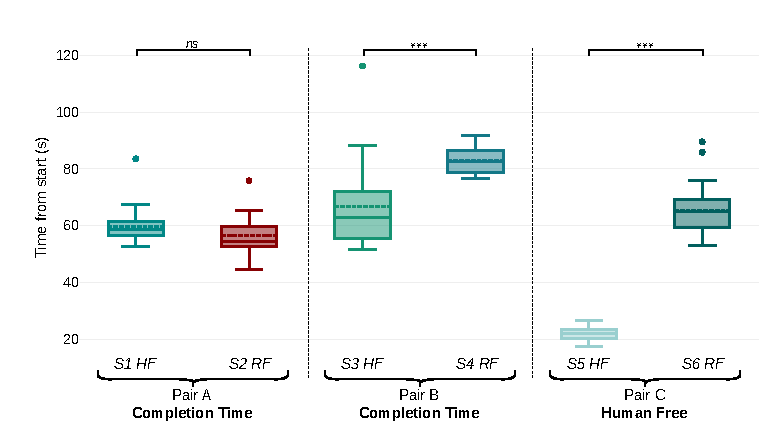
\includegraphics[width=\linewidth]{Chapter6/preferences_sastisfaction.pdf}
    \caption{Human preference satisfaction. According to the scenarios, it corresponds either to completing the task as fast as possible (Pair A and B) or being free as soon as possible (Pair C). Using t-tests for paired samples, we can identify in pair B and C the criteria of preferences is significantly better satisfied. In pair A, the difference isn't significant but the completion time is slightly shorter when using RF.}
    \label{fig:preferences_satisfaction}
\end{figure}

In this study, the human preferences consist of either finishing the collaborative task as soon as possible or being free as soon as possible while letting the robot finish alone. 
Thus, to evaluate how the human preferences were satisfied, we can measure in the first case the time to complete the task and in the second case the time after which the human can leave. 

Figure~\ref{fig:preferences_satisfaction} depicts through box plots for each pair of scenarios the corresponding relevant metric to evaluate the human preferences' satisfaction. We used t-tests for paired samples for pairwise comparison. For each pair, the tests for normal distribution suggest that the data does not significantly deviate from normality, and thus parametric tests such as t-tests can be conducted.

In Pair A, in addition to completing the stack the human wants it to be completed as soon as possible. The robot has a correct estimation of human preferences. The completion time using HF and RF are shown. The completion times in S1 and S2 are roughly similar with the respective values: $mean=59.84s SD=5.83s$ and $mean=56.64s SD=6.46s$. The completion time of Scenario 1 is higher than Scenario 2. However, a t-test for paired samples showed that this difference was not statistically significant ($p = 0.055$) and there was a small effect ($d = 0.4$) according to Cohen's \textit{d}~\cite{cohen1988concepts} (small effect = $0.2$, medium effect = $0.5$, large effect = $0.8$). Thus, the RF regime allowed the human to solve the task slightly faster than the HF regime, and thus, satisfy their preferences slightly better. 
In both scenarios, the collaboration goes smoothly, and the task is achieved without trouble.

In Pair B, the human still wants the stack to be completed as fast as possible, however, the robot has an erroneous and adversarial estimation of their preferences. This time the HF regime in S3 had lower values ($M=66.62s, SD=14.87s$) than the RF regime in S4 ($M=82.82s, SD=4.42s$). This difference is statistically significant ($p < 0.001$) and there was a large effect ($d = 1.07$). This indicates that in S4 the participants' preferences were significantly less satisfied than in S3. 
Indeed, in this pair, the robot erroneously thinks that the human wants to minimize their effort. Thus, the robot ends up trying to ``\textit{steal}'' cubes from the human to prevent them from acting, thus, minimizing their effort. With RF the human has no choice and cannot act most of the time, leading to a high completion time with a low standard deviation due to the restricted human choices leading to very similar executions. With HF the robot always acts compliantly in parallel right after the human. Hence, the human is able to pick the cubes they want and that the robot wants to pick, \textit{forcing} the robot to adapt and pick other cubes. This eventually leads to executions close to S1. However, if for any reason the human doesn't pick the cubes then the robot picks them preventing again the human from acting, explaining the high standard deviation. Comments about the feelings of the participants in each of these scenarios are given in the next subsection using the answers to the questionnaire. Overall, S4 was perceived as frustrating and S3 was perceived similarly to S1 and S2. 

In Pair C, the human prefers to be freed as soon as possible. Hence, we measured the time after which the human isn't mandatory to finish the task, i.e., the time after which the robot can finish the task alone. Scenario 5 (HF) allowed the human to be free earlier ($M=22s, SD=2.35s$) than Scenario 6 (RF) ($M=65.45s, SD=9.08s$). This difference is statistically significant ($p < 0.001$) and there was a very large effect ($d = 4.43$). This indicates that the HF regime allowed the participants to satisfy their preferences significantly better than the RF regime. 
Here, the erroneous estimation of human preferences makes the robot try to place its pink bar first, which implies that the human should place their own at the top of the stack as the last cube. Such a plan forces the human to stay until the end of the task which is in direct contradiction with the actual human preferences. Hence, after placing the yellow and red cubes concurrently, both agents tend to pick their pink bar. At this point, in S5 (HF) the robot waits for the human decision, the human can place their bar and free themselves from the task, and the robot compliantly drops its pink bar before finishing the stack alone. However, in S6 (RF), the robot doesn't wait for the human decision and places its pink bar before the human can do anything, forcing them to stay until the end to place the pink bar. As a result, the S6 values are significantly higher than S5. Moreover, the participants had various reactions to the frustrating robot action of placing the pink bar before them. Some remained passive until the end while holding their bar, others would drop it to help the robot aiming to place the bar as fast as possible anyway. These various reactions led to various executions explaining the high SD of S6.

Overall, RF tends to slightly better satisfy human preferences only when the estimation is correct (Pair A), yet, the difference wasn't significant compared the HF. On the other hand, when the estimation is erroneous, HF satisfies human preferences significantly better than RF due to how compliant the robot is when using HF. This indicates that using our model of execution instead of a simplistic baseline (RF) is beneficial for collaboration in terms of satisfaction of human preferences. 

****

\textit{We should be able to show that in scenario with similar execution, i.e. in pair A with S1 and S2, RF allows to solve the task faster, thus, human preferences are better satisfied with RF. Indeed, the S1 M1 group had higher values (M = 59,9, SD = 5,95) than the S2 M1 group (M = 56,29, SD = 6,34). A t-test for paired samples showed that this difference was statistically significant, t(23) = 2,27, p = ,033, (Small Effect)
In addition, since agents have to synchronize together at each step, we are able to measure the amount of time the human has to wait for the robot. This amount should be significantly lower when using RF than HF.
The S1 M11 (Wait ns total) group had higher values (M = 2,04, SD = 0,32) than the S2 M11 group (M = 1,29, SD = 0,36). A t-test for paired samples showed that this difference was statistically significant, t(23) = 7,4, p = <.001 (Large effect)}

\subsubsection*{Ratio human optimally}
The participants were given in every scenario an objective to satisfy, to consider as their own preferences regarding the task, and that should guide their behavior. However, in practice, the explicit actions to conduct were not given, and the participants were free to act as they would. Naturally, not all participants behaved in the same way. There were differences in the decision time of each, but also in the action decisions, leading to different execution traces.
Since different execution traces influence significantly the metrics of the timeline, it is worth discussing how the participants behaved.

First, table~\ref{tab:nb_traces} depicts the number of different execution traces per scenario and overall. There were 45 different execution when considering all scenarios, which can appear quite low compared to the $6839430$ possible plans. This also means that our exploration covers enough possibilities for this task. Additionally, it worth noticing the high number of different plans in S6 and the low number in S1. In S6, the robot acts in a quite frustrating manner which lead to various reactions of the participants. On the other hand, it seems that S1 was quite clear since participants performed only 4 different sequences of actions. It's also worth to mention that since there are only two different human objective or preferences, we would expect only 2 different optimal traces, one satisfying each objective. All other 43 other obtained traces are due either to ``wrong'' robot decision or suboptimal human decisions.

\begin{table}[h]
    \center
    \begin{tabular}{l|c|c|c|c|c|c|c|}
    \cline{2-8}
                                                                                                      & Total & S1 & S2 & S3 & S4 & S5 & S6 \\ \hline
    \multicolumn{1}{|l|}{\begin{tabular}[c]{@{}l@{}}Number of different\\ executed plan\end{tabular}} & 45    & 4  & 9  & 10 & 6  & 7  & 16 \\ \hline
    \end{tabular}
    \caption{Number of different plan executed in each scenario and overall.}
    \label{tab:nb_traces}
    \end{table}

In the same manner as for the robot, an optimal human policy is generated for each scenario (considering the actual preferences given to the participant). Hence, it is possible to check at each step if the participant performed the optimal action or not, and thus, compute an optimal ratio which is the number of optimal human actions performed divided by the total number of human actions performed. This can help us to analyze the results and can explain some outlier values. 

Though there are no significant differences between the different scenarios, some scenarios still have a lower average optimal ratio and high standard deviation, meaning that participants tend to have more varied behaviors in these specific scenarios. 
The average number of human actions per scenario is about 7, from 2 to 10. 

\begin{table}[h]
    \center
    \begin{tabular}{c|c|c|c|c|c|c|}
    \cline{2-7}
    \textbf{}                            & S1             & S2             & S3             & S4             & S5            & S6             \\ \hline
    \multicolumn{1}{|c|}{Mean}           & \textit{95.52} & \textit{95.4} & \textit{92.04} & \textit{98.03} & \textit{96.74} & \textit{87.09} \\ \hline
    \multicolumn{1}{|c|}{Std. Deviation} & \textit{7.56}  & \textit{7.78}  & \textit{8.28}  & \textit{4.58}  & \textit{7.65} & \textit{13.48} \\ \hline
    \multicolumn{1}{|c|}{Minimum}        & \textit{71.43} & \textit{71.43} & \textit{78.57} & \textit{81.25} & \textit{75}   & \textit{61.54} \\ \hline
    \multicolumn{1}{|c|}{Maximum}        & \textit{100}   & \textit{100}   & \textit{100}   & \textit{100}   & \textit{100}  & \textit{100}   \\ \hline
    \end{tabular}
    \caption{Optimal human action ratio per scenario}
    \label{tab:optimal_human_ratio}
    \end{table}



As depicted in the table~\ref{tab:optimal_human_ratio}, 
S6 has the lowest average optimal ratio and the highest std. deviation. In this scenario the robot places its own pink bar even though the human holds one already, preventing the human from placing it and forcing them to drop it back on the table. This surprising behavior seems to cause frustration and confusion which led to various human decisions and actions, and more likely to deviate from the optimal course of action. In practice, a significant amount of participants get confused and are passive during several steps after the frustrating robot action. Some even remain passive almost for the whole task, waiting for the robot to stack the cubes alone until the human pink bar has to be placed. This diversity in the participants' reaction is reflected in the high sd of S6.

The low SD of S4 is also noticeable. Indeed, here the robot tends to steal the cube from the reach of the human. This behavior prevents the human from acting, and thus, from making decisions. As a result, fewer decisions are taken by the human in this scenario which results in less possible deviation from the optimal course of action.

\subsubsection*{Decision time}
Participants' decision time fluctuates a lot. Especially with HF. Indeed, at every step, the HF robot waits for a defined amount of time to observe the human decision and acts accordingly. Any human visual signal received interrupts this timer. This amount of time will be referred to as the HF Timeout because after it is reached the robot considers the human as passive. This timeout was initially set to 3$s$ with the hypothesis that it should be quite small to allow fluent interaction. With a precise action in mind, the human is able to act first, otherwise, the robot fluently takes the lead and acts first. However, during the preliminary tests, the participants felt in a rush and oppressed by this relatively low timeout. Indeed, when they didn't have a precise action to perform when the step started, they didn't have the time to think properly and tended to be rushed by the timer progressing towards the timeout. Hence, we decided to increase the timeout from 3$s$ to 4$s$ which was felt way more comfortable. 

One could think about comparing the total (sum, cumulative) decision time over each scenario. However, since different human actions can lead to various number of steps, this isn't representative. (except in scenario with same execution, only use 100\% opti ratio?)

We compare the average human decision times which are measured similarly with HF and RF and as follows. After one participant finished one scenario, we measured their decision time on each step. To do so, we first consider for each step the time when the step begins, which is signaled with text, a gaze and a sound from the robot. Then we consider the time when the human sends a signal by either starting an action or by waving their hand. The duration between these two times is considered as the decision time of the human. Note that if the human remains passive (no signal until) for a step, no decision time is computed for this specific step. Then, we extract the average decision time of the participant on the scenario from all the computed ones, compute the standard deviation and get the maximum and minimum values. 

A one-factor analysis of variance with repeated measures showed that there was a significant difference between the variables, F = 5.99, p = <.001 with an effect size Eta squared $\eta² = 0.2$ which corresponds to a large effect.
When doing pairwise comparisons with t-tests obtain the following results.

In pair A, S1 (HF) had lower values ($M=0.66, SD=0.41$) than S2 (RF) ($M=1.04, SD=0.58$). This difference is statistically significant ($p=0.002$) with a medium effect ($d=0.68$).

In pair B, S3 (HF) had lower values ($M=0.54, SD=0.51$) than S4 (RF) ($M=0.62, SD=0.55$). This difference is not statistically significant ($p=0.551$) with a very small effect ($d=0.12$).

In pair C, S5 (HF) had lower values ($M=0.56, SD=0.11$) than S6 (RF) ($M=0.91, SD=0.46$). This difference is statistically significant ($p=0.001$) with a medium effect ($d=0.76$).

\begin{figure}
    \center
    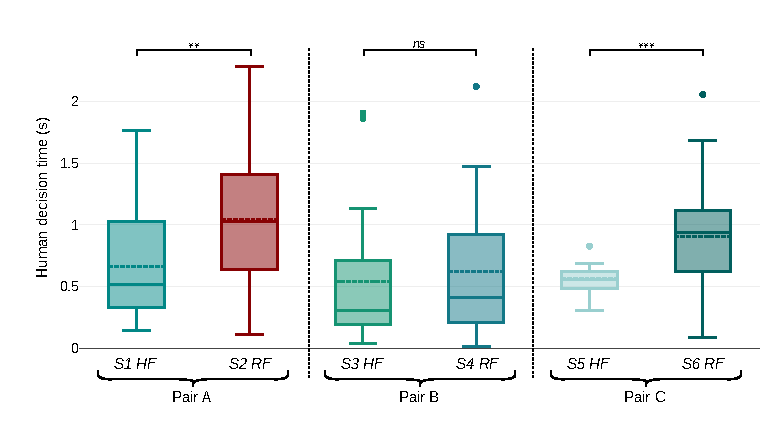
\includegraphics[width=\linewidth]{Chapter6/decision_time.pdf}
    \caption{Average human decision time in the six scenarios. This decision time tends to be lower when using HF than with RF.}
    \label{fig:decision_time}
\end{figure}

Considering the defined scenario pairs, the decision time with RF tends to be longer. However, this difference is statically significant only for pair C (S5-S6). This is expected because when the robot places the first pink bar the human gets confused and takes time to adapt to the situation. On the other hand, this is not reflected in S4 despite the similar confusing robot actions. Indeed, in S4 the robot ``steals'' cubes from the human reach which is confusing, but this prevents the human from acting and thus no decision time can be computed.  

I think the overall slower human decision time in the RF scenarios is due to the fact that the human acts after the robot. This way, the human has to pay attention to the scene and to the robot action/intentions, which is longer than only looking at the scene like in HF scenarios.   

Overall the decision time of the human is an average of about $0.72s$.


\subsubsection*{Agent actions' duration}

\begin{figure}[h]
    \center
    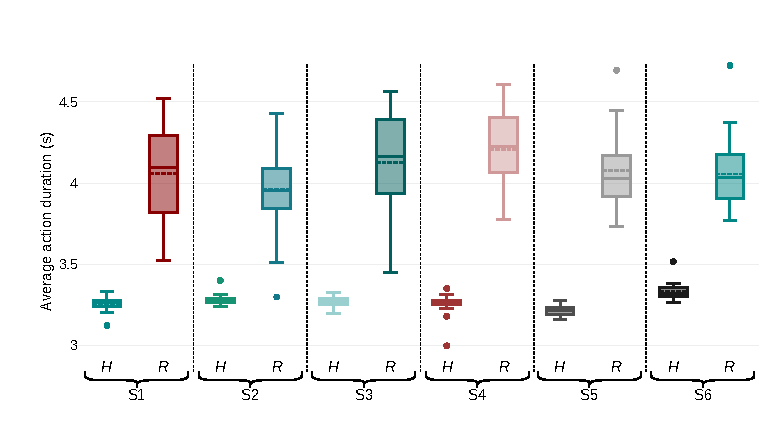
\includegraphics[width=\linewidth]{Chapter6/action_duration.pdf}
    \caption{Average action duration of the human and robot agents over the 6 scenarios, with standard deviations. Compared to the human action durations, the robot ones tend to be longer and have various durations.}
    \label{fig:action_durations}
\end{figure}

As depicted in fig.~\ref{fig:action_durations}, the human actions are in average significantly faster than the robot ones. In addition, the robot action durations tend to fluctuate more than the human one. This can be explained by the difference in motion execution between the avatar and the robot. The human has a simplified motion planner that simply moves the hand at a constant speed and in straight lines to the cubes or the stack. However, the robot uses a real motion planner to move its arm which is longer than the human motions. The motion planning process doesn't always found the same solutions, nor in the same amount of time. Meaning that both the motion planning duration and the motion execution duration can fluctuate. Here only the motion execution duration is considered in this metric. Note that to avoid having too much difference between the human and robot action durations, collisions with the dynamic objects are not considered in the robot motion planner, nor the objects' orientation. Hence, the robot can pick or place cubes from any angle and pass through the other cubes. When placing a cube its orientation is corrected. Collisions with the table where kept preventing the robot from picking cubes from below.  

Overall scenarios and steps, mean $=3.27s$ the maximum human action duration is $4.63s$ and the minimum is $2.55s$. For the robot, mean=$4.09s$, the maximum action duration is $9.09$ and the minimum duration is $1.46$.

\subsection{From questionnaires}

This section is focused on providing the results obtained by analyzing the answers to the questionnaires filled by the participants after each scenario.

To help the reader understand the following plots we list here the items of the questionnaire from the table~\ref{tab:questionnaire_answers} with their associated numeric ID in table~\ref{tab:items_id}. These IDs will be used in many plots in the x-axis to analyze the questionnaire's answers.

\begin{table}[h]
    \center
    \begin{tabular}{|cl|cl|cl|cl|}
    \hline
    \multicolumn{2}{|c|}{\textbf{Robot perception}} & \multicolumn{2}{c|}{\textbf{Interaction}} & \multicolumn{2}{c|}{\textbf{Collaboration}} & \multicolumn{2}{c|}{\textbf{Acting}} \\ \hline
    1                 & Responsive                  & 4                & Positive               & 7                & Adaptive                 & 10          & Appropriate            \\ \hline
    2                 & Competent                   & 5                & Simple                 & 8                & Useful                   & 11          & Accommodating          \\ \hline
    3                 & Intelligent                 & 6                & Clear                  & 9                & Efficient                & 12          & Predictable            \\ \hline
    \end{tabular}
    \caption{Questionnaire items with their associated IDs.}
    \label{tab:items_id}
    \end{table}


\subsubsection{Overall analysis}

We start by commenting overall questionnaire's results using some relevant average values and standard deviations before having a deeper statistical analysis in the next subsection.

\begin{figure}[h]
    \center
    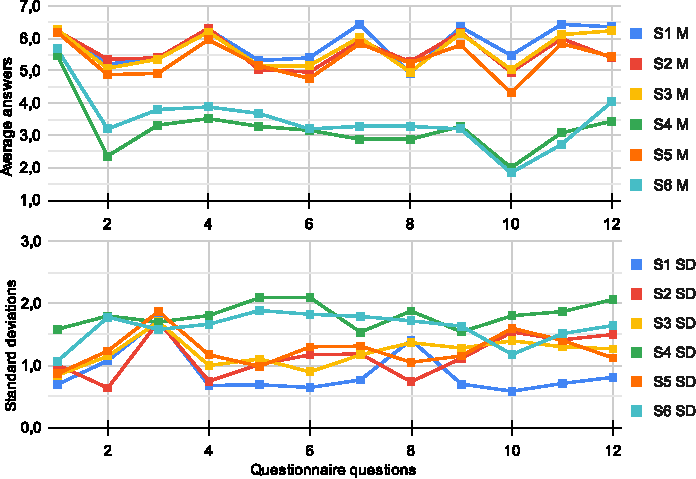
\includegraphics[width=\linewidth]{Chapter6/scenario_answers.pdf}
    \caption{W.r.t. each scenario, average answers (M, top) and standard deviations (SD, bottom) obtained for each question of the questionnaire.}
    \label{fig:scenario_answers}
\end{figure}

Figure~\ref{fig:scenario_answers} depicts the answers obtained for each question of the questionnaire w.r.t. each scenario. This figure provides a very visual overall summary of the study. On the top part, for each of the 12 questions on the x-axis, the average answers obtained are plotted for each scenario, 7 being the maximal or best value and 1 being the minimal or worst value. 
We can see that four scenarios obtained quite similar high answers whereas scenarios S4 and S6 have noticeably worse answers. Those scenarios are the Robot-First scenarios of pairs B and C where the robot has an erroneous, and even adversarial, estimation of human preferences. 
Note that question 1 (Q1) which evaluates the reactivity of the robot is the only question which answers are relatively high in every scenario.
Considering the answers to all other questions than Q1, S4 and S6 seem to deviate significantly from the other scenarios which can be analyzed as follows.
First, it means that with a correct estimation both HF and RF regimes are roughly perceived similarly. 
Second, an erroneous estimation doesn't seem to induce lower answers, and thus, despite the wrong estimation the robot in S3 and S5 is roughly perceived similarly to the one in S1 with a correct estimation.
On the other hand, when using RF, an erroneous estimation seems to have a significant detrimental impact on how the robot is perceived by the participants.
All these preliminary conclusions will be confirmed in the statistical analysis below.

It is also worth commenting on the standard deviations obtained, depicted in the bottom part of figure~\ref{fig:scenario_answers}. The standard deviations depend a lot on the scenarios and go from $0.6$ up to $2.1$. There are two noticeable facts to comment on.
First, question 3 evaluating how intelligent the robot is perceived is the only question with a relatively high SD for every scenario. Participants had various definitions of ``intelligence'' which led to a wide range of answers. Some participants evaluated the intelligence of the robot on its choices of actions, and thus, fluctuated depending on the scenario. Some others evaluated the intelligence of the robot on other criteria independent of the robot's decisions. Thus, they would rather indicate that the robot was always intelligent (or not) over all scenarios.
Additionally, we can see that the SD of S4 and S6 seem to be higher than the other scenarios.

\begin{figure}[h]
    \center
    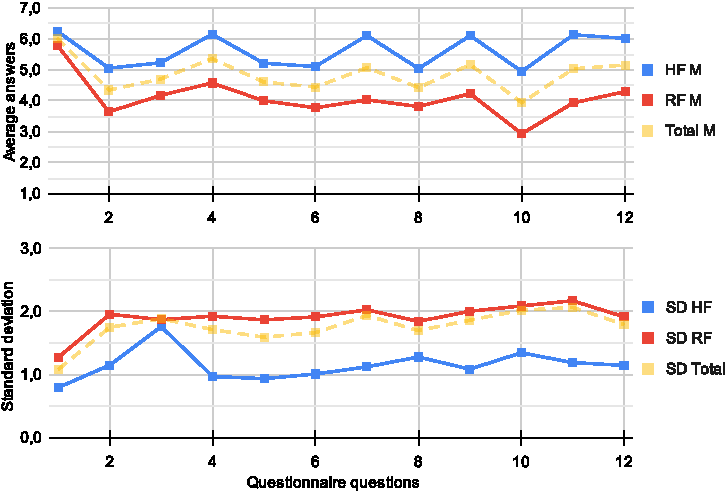
\includegraphics[width=\linewidth]{Chapter6/regime_answers.pdf}
    \caption{W.r.t. each regime of execution, average answers (M, top) and standard deviations (SD, bottom) obtained for each question of the questionnaire.}
    \label{fig:regime_answers}
\end{figure}

In contrast with the previous figure, Figure~\ref{fig:regime_answers} shows the answers obtained for each question w.r.t. to each execution regime. Indeed, the HF average answers and standard deviations, shown in blue, correspond to the union of the scenario's answers using the Human-First regime, i.e., $S1 \cup S3 \cup S5$. Similarly, the RF values, shown in red, correspond to $S2 \cup S4 \cup S6$ where the Robot-First regime is used. Additionally, the results for all scenarios combined are shown in light yellow. The results shown here can be deduced from the previous figure since we already commented on all scenarios. Yet, this new figure highlights more visually the difference between the HF and RF regimes. 

The first noticeable fact is that when using the HF regime the average answers for each question are better than when using the RF regime. Again, the only question where the answers are roughly the same regardless of the regime is when questioning the reactivity of the robot. HF's average answers are relatively high for all questions which indicates that the collaborations with HF seem to be appreciated. On the other hand, RF's answers are average (around 4) which indicates that collaborating with RF seems to be less appreciated.

Concerning the standard deviations, it is also noticeable that the answers concerning the RF regime have higher SD. This indicates that there was a wider range of answers from the participants when collaborating with the RF regime. This means that participants tend to be less certain about their answers when evaluating RF than with HF. This can be expected because when facing the HF regime the collaboration is overall quite positive, thus, participants concentrated their answers on the higher part of the scales. However, the frustrating robot actions due to the RF regime degraded the collaboration and participants had to evaluate how bad this degradation is. Some participants were more emotionally affected than others by the robot's actions, hence, it led to a wide range of answers.
Another interesting fact is that regardless of the regime, question 3 has a high standard deviation. This question evaluates the \textit{intelligence} of the robot. Participants had various definitions of intelligence which is reflected in this high SD. Indeed, some participants evaluated the robot as unintelligent because of its nature and thus regardless of its actions or the scenario. Others perceived less intelligence when the robot performed frustrating actions. 
Also, we can see that the SD regarding the reactivity of the robot is quite close and low for both regimes. This is a consequence of the very high average values regarding Q1 for both regimes.   

Eventually, I would like to insist on the average answers concerning the RF regime. Even if these answers are mediocre, it is important to note that they are not very low. In comparison, consider another robot behaving completely erratically. This robot would randomly pick and place cubes around itself. As a consequence, the robot would neither help the human nor solve the task, on the contrary, it might only disturb the human trying to achieve the task. The robot could make the task impossible to solve for the human by picking a relevant cube and never placing it, or by removing already well-placed cubes from the stack. Here, during one step, the RF regime forces the human to comply with the robot's decisions which can be frustrating. However, the robot takes into account the human action anyway and adapts accordingly its actions for the next step. This is thanks to our planning approach, common to both regimes, which explores every possible human action to generate the robot policy. Thus, we can say that our planning approach seems to benefit the collaboration and interaction between the human and the robot.

\subsubsection{ANOVA Analysis}

So far, we only conducted a preliminary analysis of the questionnaire's answers using only the average values and standard deviations. Now, a statistical analysis must be conducted to confirm the preliminary comments of the previous subsection. For each question, and thus each item of the questionnaire, we performed an analysis of the variance with repeated measures. Each analysis led to p-values $<=0.001$ indicating that there is a significant difference between the 6 scenarios. To evaluate the strength of this significant difference the effect size Eta squared $\eta^2$ has been calculated where the limits are $.01$ (small effect), $.06$ (medium effect), and $.14$ (large effect). However, ANOVA tests can only indicate if there is a significant difference between N-samples, but it is only of interest to identify between which exact group that difference exists.  In the Bonferroni post-hoc test in a repeated measures ANOVA, multiple t-tests are calculated for dependent samples. However, the problem with multiple testing is that the so-called alpha error (the false rejection of the null hypothesis) increases with the number of tests. To counteract this, the Bonferroni post-hoc test calculates the obtained p-values times the number of tests. The obtained p-values indicate in a pairwise manner between which samples the significant difference exists. The results from the ANOVA and Bonferroni post-hoc test are shown in table~\ref{tab:questionnaire_answers}.

\begin{sidewaystable}
    \center
        \begin{tabular}{c|cc|ccccccccccccccc|}
        \cline{2-18}
        \multicolumn{1}{l|}{}                        & \multicolumn{2}{c|}{\textbf{ANOVA}}                                 & \multicolumn{15}{c|}{\textbf{Bonferroni Post hoc tests}}                                                                                                                                                                                                                                                                                                                                                                                                                                                                                                                                                                        \\ \cline{2-18} 
        \multicolumn{1}{l|}{}                        & \multicolumn{1}{c|}{p}            & $\eta^2$               & \multicolumn{1}{c|}{1-2}         & \multicolumn{1}{c|}{1-3}         & \multicolumn{1}{c|}{\textbf{1-4}}          & \multicolumn{1}{c|}{1-5}                  & \multicolumn{1}{c|}{\textbf{1-6}}          & \multicolumn{1}{c|}{2-3}         & \multicolumn{1}{c|}{\textbf{2-4}}          & \multicolumn{1}{c|}{2-5}         & \multicolumn{1}{c|}{\textbf{2-6}}          & \multicolumn{1}{c|}{\textbf{3-4}}          & \multicolumn{1}{c|}{3-5}                 & \multicolumn{1}{c|}{\textbf{3-6}}          & \multicolumn{1}{c|}{\textbf{4-5}}          & \multicolumn{1}{c|}{4-6}         & \textbf{5-6}          \\ \hline
        \multicolumn{1}{|c|}{Responsive}             & \multicolumn{1}{c|}{\textit{***}} & \textit{0.16}          & \multicolumn{1}{c|}{\textit{ns}} & \multicolumn{1}{c|}{\textit{ns}} & \multicolumn{1}{c|}{\textit{ns}}           & \multicolumn{1}{c|}{\textit{ns}}          & \multicolumn{1}{c|}{\textit{ns}}           & \multicolumn{1}{c|}{\textit{ns}} & \multicolumn{1}{c|}{\textit{ns}}           & \multicolumn{1}{c|}{\textit{ns}} & \multicolumn{1}{c|}{\textit{ns}}           & \multicolumn{1}{c|}{\textit{ns}}           & \multicolumn{1}{c|}{\textit{ns}}         & \multicolumn{1}{c|}{\textit{ns}}           & \multicolumn{1}{c|}{\textit{ns}}           & \multicolumn{1}{c|}{\textit{ns}} & \textit{ns}           \\ \hline
        \multicolumn{1}{|c|}{Competent}              & \multicolumn{1}{c|}{\textit{***}} & \textit{0.49}          & \multicolumn{1}{c|}{\textit{ns}} & \multicolumn{1}{c|}{\textit{ns}} & \multicolumn{1}{c|}{\textit{\textbf{***}}} & \multicolumn{1}{c|}{\textit{ns}}          & \multicolumn{1}{c|}{\textit{\textbf{***}}} & \multicolumn{1}{c|}{\textit{ns}} & \multicolumn{1}{c|}{\textit{\textbf{***}}} & \multicolumn{1}{c|}{\textit{ns}} & \multicolumn{1}{c|}{\textit{\textbf{***}}} & \multicolumn{1}{c|}{\textit{\textbf{***}}} & \multicolumn{1}{c|}{\textit{ns}}         & \multicolumn{1}{c|}{\textit{\textbf{**}}}  & \multicolumn{1}{c|}{\textit{\textbf{***}}} & \multicolumn{1}{c|}{\textit{ns}} & \textit{\textbf{*}}   \\ \hline
        \multicolumn{1}{|c|}{Intelligent}            & \multicolumn{1}{c|}{\textit{***}} & \textit{0.33}          & \multicolumn{1}{c|}{\textit{ns}} & \multicolumn{1}{c|}{\textit{ns}} & \multicolumn{1}{c|}{\textit{\textbf{**}}}  & \multicolumn{1}{c|}{\textit{ns}}          & \multicolumn{1}{c|}{\textit{\textbf{*}}}   & \multicolumn{1}{c|}{\textit{ns}} & \multicolumn{1}{c|}{\textit{\textbf{**}}}  & \multicolumn{1}{c|}{\textit{ns}} & \multicolumn{1}{c|}{\textit{\textbf{**}}}  & \multicolumn{1}{c|}{\textit{\textbf{**}}}  & \multicolumn{1}{c|}{\textit{ns}}         & \multicolumn{1}{c|}{\textit{\textbf{***}}} & \multicolumn{1}{c|}{\textit{\textbf{*}}}   & \multicolumn{1}{c|}{\textit{ns}} & \textit{\textbf{*}}   \\ \hline
        \multicolumn{1}{|c|}{\textbf{Positive}}      & \multicolumn{1}{c|}{\textit{***}} & \textit{\textbf{0.65}} & \multicolumn{1}{c|}{\textit{ns}} & \multicolumn{1}{c|}{\textit{ns}} & \multicolumn{1}{c|}{\textit{\textbf{***}}} & \multicolumn{1}{c|}{\textit{ns}}          & \multicolumn{1}{c|}{\textit{\textbf{***}}} & \multicolumn{1}{c|}{\textit{ns}} & \multicolumn{1}{c|}{\textit{\textbf{***}}} & \multicolumn{1}{c|}{\textit{ns}} & \multicolumn{1}{c|}{\textit{\textbf{***}}} & \multicolumn{1}{c|}{\textit{\textbf{***}}} & \multicolumn{1}{c|}{\textit{ns}}         & \multicolumn{1}{c|}{\textit{\textbf{***}}} & \multicolumn{1}{c|}{\textit{\textbf{***}}} & \multicolumn{1}{c|}{\textit{ns}} & \textit{\textbf{***}} \\ \hline
        \multicolumn{1}{|c|}{Simple}                 & \multicolumn{1}{c|}{\textit{***}} & \textit{0.34}          & \multicolumn{1}{c|}{\textit{ns}} & \multicolumn{1}{c|}{\textit{ns}} & \multicolumn{1}{c|}{\textit{\textbf{**}}}  & \multicolumn{1}{c|}{\textit{ns}}          & \multicolumn{1}{c|}{\textit{\textbf{**}}}  & \multicolumn{1}{c|}{\textit{ns}} & \multicolumn{1}{c|}{\textit{\textbf{**}}}  & \multicolumn{1}{c|}{\textit{ns}} & \multicolumn{1}{c|}{\textit{ns}}           & \multicolumn{1}{c|}{\textit{\textbf{*}}}   & \multicolumn{1}{c|}{\textit{ns}}         & \multicolumn{1}{c|}{\textit{\textbf{*}}}   & \multicolumn{1}{c|}{\textit{\textbf{**}}}  & \multicolumn{1}{c|}{\textit{ns}} & \textit{\textbf{*}}   \\ \hline
        \multicolumn{1}{|c|}{Clear}                  & \multicolumn{1}{c|}{\textit{***}} & \textit{0.41}          & \multicolumn{1}{c|}{\textit{ns}} & \multicolumn{1}{c|}{\textit{ns}} & \multicolumn{1}{c|}{\textit{\textbf{***}}} & \multicolumn{1}{c|}{\textit{ns}}          & \multicolumn{1}{c|}{\textit{\textbf{***}}} & \multicolumn{1}{c|}{\textit{ns}} & \multicolumn{1}{c|}{\textit{\textbf{**}}}  & \multicolumn{1}{c|}{\textit{ns}} & \multicolumn{1}{c|}{\textit{\textbf{***}}} & \multicolumn{1}{c|}{\textit{\textbf{***}}} & \multicolumn{1}{c|}{\textit{ns}}         & \multicolumn{1}{c|}{\textit{\textbf{***}}} & \multicolumn{1}{c|}{\textit{\textbf{*}}}   & \multicolumn{1}{c|}{\textit{ns}} & \textit{\textbf{**}}  \\ \hline
        \multicolumn{1}{|c|}{\textbf{Adaptive}}      & \multicolumn{1}{c|}{\textit{***}} & \textit{\textbf{0.62}} & \multicolumn{1}{c|}{\textit{ns}} & \multicolumn{1}{c|}{\textit{ns}} & \multicolumn{1}{c|}{\textit{\textbf{***}}} & \multicolumn{1}{c|}{\textit{ns}}          & \multicolumn{1}{c|}{\textit{\textbf{***}}} & \multicolumn{1}{c|}{\textit{ns}} & \multicolumn{1}{c|}{\textit{\textbf{***}}} & \multicolumn{1}{c|}{\textit{ns}} & \multicolumn{1}{c|}{\textit{\textbf{***}}} & \multicolumn{1}{c|}{\textit{\textbf{***}}} & \multicolumn{1}{c|}{\textit{ns}}         & \multicolumn{1}{c|}{\textit{\textbf{***}}} & \multicolumn{1}{c|}{\textit{\textbf{***}}} & \multicolumn{1}{c|}{\textit{ns}} & \textit{\textbf{***}} \\ \hline
        \multicolumn{1}{|c|}{Useful}                 & \multicolumn{1}{c|}{\textit{***}} & \textit{0.43}          & \multicolumn{1}{c|}{\textit{ns}} & \multicolumn{1}{c|}{\textit{ns}} & \multicolumn{1}{c|}{\textit{\textbf{***}}} & \multicolumn{1}{c|}{\textit{ns}}          & \multicolumn{1}{c|}{\textit{\textbf{*}}}   & \multicolumn{1}{c|}{\textit{ns}} & \multicolumn{1}{c|}{\textit{\textbf{***}}} & \multicolumn{1}{c|}{\textit{ns}} & \multicolumn{1}{c|}{\textit{\textbf{***}}} & \multicolumn{1}{c|}{\textit{\textbf{***}}} & \multicolumn{1}{c|}{\textit{ns}}         & \multicolumn{1}{c|}{\textit{\textbf{**}}}  & \multicolumn{1}{c|}{\textit{\textbf{***}}} & \multicolumn{1}{c|}{\textit{ns}} & \textit{\textbf{***}} \\ \hline
        \multicolumn{1}{|c|}{\textbf{Efficient}}     & \multicolumn{1}{c|}{\textit{***}} & \textit{\textbf{0.62}} & \multicolumn{1}{c|}{\textit{ns}} & \multicolumn{1}{c|}{\textit{ns}} & \multicolumn{1}{c|}{\textit{\textbf{***}}} & \multicolumn{1}{c|}{\textit{ns}}          & \multicolumn{1}{c|}{\textit{\textbf{***}}} & \multicolumn{1}{c|}{\textit{ns}} & \multicolumn{1}{c|}{\textit{\textbf{***}}} & \multicolumn{1}{c|}{\textit{ns}} & \multicolumn{1}{c|}{\textit{\textbf{***}}} & \multicolumn{1}{c|}{\textit{\textbf{***}}} & \multicolumn{1}{c|}{\textit{ns}}         & \multicolumn{1}{c|}{\textit{\textbf{***}}} & \multicolumn{1}{c|}{\textit{\textbf{***}}} & \multicolumn{1}{c|}{\textit{ns}} & \textit{\textbf{***}} \\ \hline
        \multicolumn{1}{|c|}{\textbf{Appropriate}}   & \multicolumn{1}{c|}{\textit{***}} & \textit{\textbf{0.62}} & \multicolumn{1}{c|}{\textit{ns}} & \multicolumn{1}{c|}{\textit{ns}} & \multicolumn{1}{c|}{\textit{\textbf{***}}} & \multicolumn{1}{c|}{\textit{\textbf{**}}} & \multicolumn{1}{c|}{\textit{\textbf{***}}} & \multicolumn{1}{c|}{\textit{ns}} & \multicolumn{1}{c|}{\textit{\textbf{***}}} & \multicolumn{1}{c|}{\textit{ns}} & \multicolumn{1}{c|}{\textit{\textbf{***}}} & \multicolumn{1}{c|}{\textit{\textbf{***}}} & \multicolumn{1}{c|}{\textit{ns}}         & \multicolumn{1}{c|}{\textit{\textbf{***}}} & \multicolumn{1}{c|}{\textit{\textbf{***}}} & \multicolumn{1}{c|}{\textit{ns}} & \textit{\textbf{***}} \\ \hline
        \multicolumn{1}{|c|}{\textbf{Accommodating}} & \multicolumn{1}{c|}{\textit{***}} & \textit{\textbf{0.68}} & \multicolumn{1}{c|}{\textit{ns}} & \multicolumn{1}{c|}{\textit{ns}} & \multicolumn{1}{c|}{\textit{\textbf{***}}} & \multicolumn{1}{c|}{\textit{ns}}          & \multicolumn{1}{c|}{\textit{\textbf{***}}} & \multicolumn{1}{c|}{\textit{ns}} & \multicolumn{1}{c|}{\textit{\textbf{***}}} & \multicolumn{1}{c|}{\textit{ns}} & \multicolumn{1}{c|}{\textit{\textbf{***}}} & \multicolumn{1}{c|}{\textit{\textbf{***}}} & \multicolumn{1}{c|}{\textit{ns}}         & \multicolumn{1}{c|}{\textit{\textbf{***}}} & \multicolumn{1}{c|}{\textit{\textbf{***}}} & \multicolumn{1}{c|}{\textit{ns}} & \textit{\textbf{***}} \\ \hline
        \multicolumn{1}{|c|}{Predictable}            & \multicolumn{1}{c|}{\textit{***}} & \textit{0.45}          & \multicolumn{1}{c|}{\textit{ns}} & \multicolumn{1}{c|}{\textit{ns}} & \multicolumn{1}{c|}{\textit{\textbf{***}}} & \multicolumn{1}{c|}{\textit{\textbf{**}}} & \multicolumn{1}{c|}{\textit{\textbf{***}}} & \multicolumn{1}{c|}{\textit{ns}} & \multicolumn{1}{c|}{\textit{\textbf{*}}}   & \multicolumn{1}{c|}{\textit{ns}} & \multicolumn{1}{c|}{\textit{\textbf{*}}}   & \multicolumn{1}{c|}{\textit{\textbf{***}}} & \multicolumn{1}{c|}{\textit{\textbf{*}}} & \multicolumn{1}{c|}{\textit{\textbf{***}}} & \multicolumn{1}{c|}{\textit{\textbf{**}}}  & \multicolumn{1}{c|}{\textit{ns}} & \textit{\textbf{**}}  \\ \hline
        \end{tabular}
        \caption{Significant differences in the questionnaire answers between the different scenarios. For each item of the questionnaire are shown the overall p-value and $\eta^2$ (effect size) obtained after an ANOVA. Additionally, the p values obtained after conducting Bonferroni Post-hoc-Tests are shown to identify in a pair-wise manner which scenarios were significantly different from others. As depicted, scenarios 4 and 6 are distinguishable from the others and their evaluation are significantly different on all the measured aspect (expect reactivity).}
        \label{tab:questionnaire_answers}
\end{sidewaystable}

As suggested by the preliminary analysis, the Reactivity of the robot is the item with the lowest difference. The ANOVA indicates that answers regarding the reactivity are significantly different with a large effect over the 6 scenarios. However, compared to other items, the effect size $\eta^2$ is quite low indicating that this difference is less significant than for other items. Also, the Bonferroni post-hoc test wasn't able to identify where exactly the difference exists, which means again that this difference isn't very significant in the end. 

Besides reactivity, all other items have large significant differences according to the scenario which can be exploited using the Bonferroni post-hoc test. 
Indeed, the pairwise comparisons indicate the existence of major significant differences for every question in the following pairs: S1-S4, S1-S6, S2-S4, S2-S6, S3-S4, S3-S6, S4-S5, and S5-S6 (in bold in the table). Having in mind that S4 and S6 are the two scenarios using Robot-First with erroneous estimations, we can see that erroneous estimation with RF systematically leads to significant differences compared to all other scenarios using HF or RF with a correct estimation (S4-S1, S4-S2, S4-S3, S4-S5, and S6-S1, S6-S2, S6-S3, S6-S5). This is a clear indicator that the RF regime is very sensitive to the estimation of the human preferences and thus an erroneous estimation is significantly detrimental to the collaboration and the overall interaction. 

Only a few other significant differences exist and are in S1-S5 and S3-S5. Indeed, in S5, the robot's actions were perceived as more or less significantly less appropriate ($p=0.004$) and predictable ($p=0.004$) than in S1, slightly less predictable ($p=0.017$) than in S3. Indeed, in S5 the HF robot surprisingly picks up its pink bar while the human picks up its own whereas the human wants to place their bar to be freed from the task. Using HF allows the human to place their bar anyway, but the robot actions were therefore perceived as less predictable and appropriate than in S1 or S3. 
We can also notice that despite S3 having an erroneous estimation in contrast to S1, there is no significant difference in answers for each question between S1 and S3. 
This indicates that using the HF regime allows the robot to be way more robust to erroneous estimation than RF. However, the few existing significant differences among the HF scenarios indicate that an erroneous estimation is still noticeable and can still have a detrimental influence. Thus, the robot cannot fully rely on being reactive and compliant to human actions. Estimating the human preferences accurately to plan appropriately the robot's actions is mandatory for optimal collaboration.

Looking at the eta squared $\eta^2$ of every question, one can notice that we can group the items into 4 groups. 
% First, the Reactivity item is alone with the lowest effect size ($\eta^2=0.16$). This group doesn't really help to distinguish the regimes. 
% Secondly, with an effect size of around $\eta^2 \simeq 0.33$, we can state that when using RF the robot was perceived as slightly less intelligent and the interaction as slightly less simple than when using HF. 
% Then, with an effect size of around $\eta^2 \simeq 0.45$, we can state that when using RF the robot was perceived as moderately less competent, the interaction as moderately less clear, the collaboration as moderately less useful, and the robot actions as moderately less predictable. 
% Eventually, with an effect size of around $\eta^2 \simeq 0.64$, when using the RF regime the interaction was perceived as significantly less positive, the collaboration as significantly less adaptive and efficient, and the robot actions as significantly less appropriate and less accommodation. 
% Since the five items from the last group are the ones with the highest effect size, they can be seen as the main characteristics differentiating the HF from the RF regimes and thus are highlighted in the table.
\begin{enumerate}
    \item $\eta^2=0.16$: First, the Reactivity item is alone with the lowest effect size. This group doesn't help to distinguish the regimes. 
    \item $\eta^2 \simeq 0.33$: Secondly, we can state that when using RF the robot was perceived as slightly less intelligent and the interaction as slightly less simple than when using HF. 
    \item $\eta^2 \simeq 0.45$: Then, due to the moderate effect size, we can state that when using RF the robot was perceived as moderately less competent, the interaction as moderately less clear, the collaboration as moderately less useful, and the robot actions as moderately less predictable. 
    \item $\eta^2 \simeq 0.64$: Eventually, with a high effect size, when using the RF regime the interaction was perceived as significantly less positive, the collaboration as significantly less adaptive and efficient, and the robot actions as significantly less appropriate and less accommodation. Since the five items from the last group are the ones with the highest effect size, they can be seen as the main characteristics differentiating the HF from the RF regimes and thus are highlighted in the table.
\end{enumerate}

% ***

% Except reactive, all Q significantly vary according to scenarios

% S4 and S6 are significantly different from others

% with effect size talk about Q that are most diff [~0.6-0.7] (Positive, Adaptive, Efficient, Appropriate, Accommodating), 

% medium diff [~0.4-0.5] (Competent, Clear, Useful, Predictable), 

% low diff [~0.3] (Intelligent, Simple) 

% and lowest [0.16] (Reactive)

% Talk about the few other diff (1-5, )

% *****

% Some questions have large standard deviations, such as about the perceived ``Intelligence'', but often only on specific scenarios.

% The ``Reactive'' answers are overall the same, whatever execution regime and scenario. 
% Overall, based on an ANalysis Of the VAriance with repeated measures (ANOVA), all other answers than ``Reactive'' vary significantly. Post-tests show that the main differences come from scenarios S4 and S6. Those two scenarios correspond to ones where the robot has an incorrect estimation of the human preferences and is following the \textit{Robot-First} execution regime. This indicates that all HF behaviors are perceived similarly despite the erroneous estimation of the robot. It also indicates that the RF scenario with correct estimation is positively perceived, but an erroneous estimation has a significant impact on the answers when using RF.  

% Except for the ``Reactive'' aspect, answers about RF have a larger standard deviation. Thus, participants tend to be more indecisive regarding RF than HF.

% About ``Reactive''. A Bonferroni Post hoc test was used to compare the groups in pairs to find out which was significantly different.
% Despite the significant difference in the ANOVA, no pairwise group comparison was significant in the Bonferroni Post hoc test; all p values were greater than 0,05. 

% S4 and S6 received significantly worse answers than the other scenarios. It is interesting to notice that in a pair-wise manner, all other scenarios 

% We notice very few significant differences on HF only.

% In table \ref{tab:questionnaire_answers} there almost only significant differences in pairs involving S4 and S6. The only few other differences are the following. 
% S1 is significantly more appropriate than S5. And S5 is significantly less predictable than S1 and S3

% \begin{figure}[h]
%     \centering
%     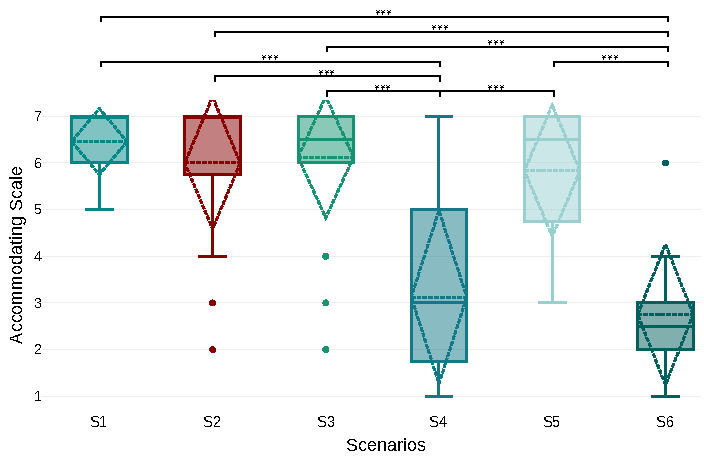
\includegraphics[width=\linewidth]{Chapter6/signif_accommo.pdf}
%     \caption{Accommodating Interaction Scale with ANOVA + Post-hoc-Tests}
%     \label{fig:accommodating_scale_anova}
% \end{figure}

\subsection{From comments}

At the end of the experiment, every participant was asked two questions gathering their general impressions. First, they were asked to comment on the overall experiment and robot interaction they just had. Secondly, participants were asked to indicate which scenario they preferred the most and the least. 

Participants' comments concern several aspects of the experiment and are worth discussing. Overall, the comments confirm the outcome of the statistical analysis, and they also provide some feedback about the overall experiment protocol and conditions, especially regarding the simulator itself. The comments are discussed per categories below. 

\textbf{TODO: Try to add more argumentation and links to previous results, be less descriptive...}

\subsubsection{Simulation}
First, most of the participants found the experiment and the simulation as a good experience. They felt committed and active during the different scenarios. 
The simulation has been described several times as clear, simple, pleasant, intuitive, captivating, and funny. 
Some participants mentioned that it was like a video game and enjoyed it. 
These comments suggest that collaborating with a simulated robot has been appreciated, and they raise the question if the participant had felt the same way in an experiment with a real robot. 

\subsubsection{Display}
Some participants think that the simulation display had too much information (goal + scene + text prompt), and a few had trouble reading the text prompt. Yet, the robot can be seen well. Indeed, the text prompts could be a bit fast and written white on black, which can be disturbing when not used to. However, I believe this didn't affect much the executions, maybe slightly the decision times. 

\subsubsection{General}
A few participants would have appreciated the robot giving instructions and guidance regarding the actions to perform. This is linked to another comment saying that using the Robot-Fist regime with correct estimation felt better because makes the task simpler. If the human trusts the robot, it can be appreciated to let the robot compute the optimal plan and just follow the robot's instructions, lowering the cognitive load of the human. Indeed, some participants consider that they made mistakes and that they could have acted in a better way in some scenarios. 

\subsubsection{Steps}
The step synchronization wasn't appreciated by everyone. Some participants found this kind of synchronization useful as it structured the collaboration. However, many others found this a bit confusing at first and frustrating because they had to wait for the robot's actions to be done before being able to act again.

\subsubsection{Task}
The task was found clear and quite simple. One participant said that they felt significant emotions such as satisfaction and frustration and that if the task was less abstract and more real, these emotions would have been enhanced. Moreover, another participant said that in such simple tasks, humans tend to think they know better how to solve the task than the robot. Thus, the robot should follow human decisions in such cases, with a hierarchy relation. A few participants also mentioned that performing the last action, i.e. placing the last cube, is very satisfying. These people liked the robot adapting to allow them to do so. 
The fact that both agents must perform actions to solve the task makes the collaboration relevant and useful. 

\subsubsection{Action}
Many participants said that not being able to pick cubes in advance isn't natural and, at first, it is confusing, frustrating, and a bit complicated. Yet, they also said that they got used to it quite fast. One also said that they felt obliged to act at every step. Indeed, a majority of the participants were signaling their passivity to the robot even when they were not able to act. 
About the movements, one participant stated that the actions were stiff and rigid, in contrast to being able to drag and drop the cubes thanks to the physics simulation. Additionally, the lack of collision with the cubes felt a bit unrealistic but not very confusing.
On the other hand, another participant said that the robot's movements seem real. This is probably due to the fact we used an online motion planner to move the robot arm, thus, the movements were not always optimal.

\subsubsection{Objective}
A few participants said that the objective of "trying to be free early" is a bit frustrating since they would like to keep acting, even if not necessary. It was hard for them to consider this objective as their personal preference, and thus, to act accordingly. 
Additionally, one participant mentioned that Scenario 5 creates double satisfaction: being free early (preferences) and the task is fulfilled.

\subsubsection{Regimes}
One participant said that they didn't see much difference between the two execution regimes HF and RF. The same participant couldn't indicate which scenario they preferred at the end. Moreover, some participants also indicated that the difference between HF and RF was unclear at first. However, once used to the task and the scenarios, the difference becomes clearer and before the end of the experiment, most of the participants had a clear idea of each regime, and even apprehended the RF one.

\subsubsection{Being in control}
Participants indicated that when using HF they felt in control, free to decide which action they performed, and that the robot was adapting to their decisions and actions, which was appreciated. In contrast, when using RF, participants didn't feel in control and were forced to adapt to the robot's decisions. Even when the robot's decisions are good, the lack of control is uncomfortable. One participant stated that they disliked when the robot took initiative because the robot could be wrong. 

\subsubsection{Human-First (HF) regime}
Most of the participants enjoyed the HF regime and stated that they were able to fulfill their objective with it. Some comments qualify the HF regime as slower than RF and sometimes inconsistent. The latter is mostly referring to the robot picking up the pink bar in S5. However, especially when used to it, HF has been qualified as smooth, efficient, interesting, predictable, and less frustrating than RF. Several participants mentioned that they enjoyed being able to predict the robot's behavior, proving that having predictable behavior is crucial for a seamless collaboration. It has been mentioned that HF makes less wrong choices than RF.
Moreover, some participants said that compared to the RF regime with a correct estimation HF is less efficient, however, in pairs B and C HF is more efficient than RF.

\subsubsection{Robot-First (RF) regime}
RF, bad, not in control, bad choices: having to drop bar + using common resources first

Every participant had an overall negative opinion regarding the RF regime. The latter has been qualified as very frustrating, confusing, constraining, unpredictable, inefficient, and even adversarial. A significant number of participants stated that to finish the task quickly RF could be great, fast, efficient, and less cognitively demanding, despite the lack of control. Also, a few participants noticed that even if during a specific step the human is forced to comply with the robot's actions, in the next step the robot takes into account the human action and adapts its behavior. 
However, it has been said that RF doesn't consider the human's objective or preferences. Participants really disliked when the robot forced them to drop a cube back on the table (pink bar in S6) and when the robot picked cubes in the middle zone instead of its own zone. The latter was perceived as the robot stealing the cubes from the human.
Due to those frustrating robot actions, the RF regime was putting the participants in an adversarial setup and the robots were explicitly qualified as ``enemies''. Some participants said that they were more focused on preventing the robot's mistakes than on the actual task.


\section{Discussion}

\textbf{TODO: to develop}

There are several elements to discuss in this study, including several participants' comments.

\begin{itemize}
    \item simulation to real life ? what would it take ? different results ? One in between solution is using VR. Requires flexible execution scheme like described in limitations in chapter \ref{chap:5}.
    \item Simu not realistic enough (pass trough cubes, no orientation, etc..): since focused on decisions, was enough but we could have done better. 
    \item Text prompt: Which info to prompt ? when ? and how (sometimes hard to read). maybe vocal would have been better ? Here no specific study has been conducted, we simply show to the participants some inner state of the robot (waiting for human, acting, identifying human action, ...)
    \item A different task ? only manipulation ? no navigation ?  Here the task carefully design to not be too long and still be significantly influenced by pairs of pref-esti
    \item Using an additional baseline with an erratic robot could have helped showing RF not so bad. 
\end{itemize}

\section{Conclusion}

% Our purpose was to validate thanks to this study both the overall planning approach as well as the model of execution Human-First which is key to our approach. 

% After statistically analyzing the execution log data as objective metrics, and the questionnaire answers and participants' comments as subjective metrics, we can confidently state that this study successfully validates both our planning approach and our model of execution. 

% Indeed, we have solid proof that the HF regime has been preferred by the participants because of the control it gives to the human. The robot is perceived as accommodating, adaptive, and acting appropriately while being predictable. HF also helps to better satisfy the human inner preferences which makes it more robust to erroneous estimations and thus more enjoyable. 
% On the other hand, we also show how the RF regime can be appreciated a lot when estimating correctly human preferences, but we also show how erroneous estimations are strongly detrimental to collaboration and interaction when using the RF regime. 
% Hence, the Human-First regime is preferred and allows for achieving smooth, efficient, and positive collaborations.
% Yet, we also show that even when using the Robot-First regime the robot is able to always solve the task with the human, thus, it is always found useful. It also still adapts to human actions in the next step thanks to our policy format. This means that our planning approach is still efficient and appropriate for this context. 

% ****

\textbf{TODO: be more specific which conclusion come from which data? preferences satisfaction from log, adjectives from questionnaire, from comments ? confirmation + discussion materials.}

Thanks to this study, we aimed to validate the overall planning approach and the model of execution Human-First, which is critical to our approach. 

After statistically analyzing the execution log data as objective metrics and the questionnaire answers and participants' comments as subjective metrics, we can confidently state that this study successfully validates both our planning approach and our model of execution. 

Indeed, we have solid proof that the  HF regime gives humans control over the execution, which was significantly appreciated. The participants perceived the robot as accommodating, adaptive, and acting appropriately while being predictable. HF also helps to satisfy better human inner preferences, which makes it more robust to erroneous estimations and thus more enjoyable. 
On the other hand, we show how the RF regime can be greatly appreciated when estimating human preferences correctly. However, we demonstrate how erroneous estimations strongly harm collaboration and interaction using the RF regime. 
Hence, the Human-First regime is preferred and allows for achieving smooth, efficient, and positive collaborations.
Nevertheless, thanks to our planning approach, we also show that the RF regime always solves the task with humans, and thus, it is always helpful. Additionally, it also always adapts to human action in the next step. 
